\chapter{坐标变换}
\section{坐标轴的平移}

首先必须明确，点的坐标和曲线的方程都是对特定的坐标系而言的.如果建立的坐标系不同，点的坐标和曲线的方程也就不同. 例如，图
    4.1中点$O'$和$\odot O'$在坐标系$xOy$中的坐标和方程分别是$(3,4)$和
    \begin{equation}
        (x-3)^2+(y-4)^2=4\tag{1}
    \end{equation}
    
    如果把坐标轴$Ox$和$Oy$分别平行移动到$O'x'$与$O'y'$，那么，就得到了一个新的坐标系$x'O'y'$，在这个新坐标系中，点$O'$的坐标和$\odot O'$的方程却变成了
\begin{equation}
    (0,0)\quad \text{和}\quad x'^{2}+y'^{2}=4  \tag{2}
\end{equation}

这种把坐标轴平行移动的变换叫做\textbf{坐标轴的平移变换}（简称\textbf{移轴}）.显然，在这种变换下坐标轴的方向和单位长均未改变，而仅仅是改变了原点的位置.

\noindent
\begin{minipage}{.48\textwidth}
    \centering
   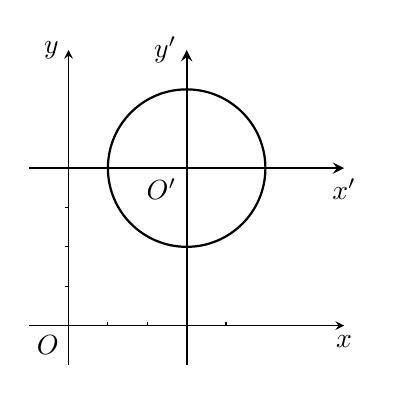
\begin{tikzpicture}[>=stealth, scale =.5]
\draw[->](-1,0)--(7,0)node[below]{$x$};
\draw[->](0,-1)--(0,7)node[left]{$y$};
\foreach \x in {1,2,3,4}
{
    \draw(\x,0)--(\x,.1);
    \draw(0,\x)--(-.1,\x);
}
\draw[->, thick](-1,4)--(7,4)node[below]{$x'$};
\draw[->, thick](3,-1)--(3,7)node[left]{$y'$};
\draw[thick](3,4)node[below left]{$O'$}circle(2);
\node[below left]{$O$};

\end{tikzpicture}
\captionof{figure}{}
\end{minipage}
\hfill
\begin{minipage}{.48\textwidth}
    \centering
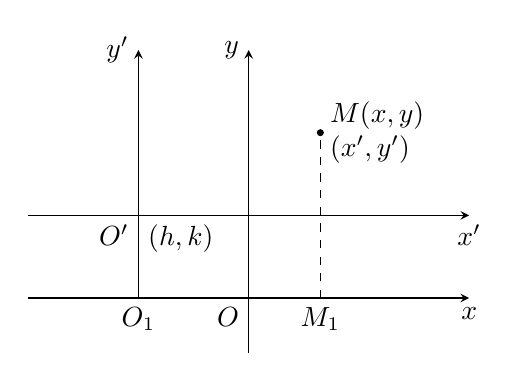
\begin{tikzpicture}[>=stealth, scale =.7]
\draw[->](-4,0)--(4,0)node[below]{$x$};
\draw[->](-4,1.5)--(4,1.5)node[below]{$x'$};
\draw[->](0,-1)--(0,4.5)node[left]{$y$};
\draw[->](-2,0)node[below]{$O_1$}--(-2,4.5)node[left]{$y'$};
\node[below left]{$O$};
\node at (-2,1.5)[below left]{$O'$};
\draw[dashed](1.3,0)node[below]{$M_1$}--(1.3,3)node[right, text width =2cm, align=left]{$M(x,y)$\\$(x',y')$};
\node at (-2,1.5)[below right]{$(h,k)$};
\draw[fill](1.3,3) circle(1.5pt);
\end{tikzpicture}
\captionof{figure}{}
\end{minipage}

观察上面得到的(1)和(2)可以看出，把坐标系$xOy$平移到$x'O'y'$以后，$\odot O'$的方程被简化了. 这启示我们：适当地进行移轴可以化简曲线的方程. 这正是移轴的重要作用.

下面研究在坐标轴的平移变换下，点的坐标和曲线的方程变化的规律. 事实上，我们只须找出坐标平面上任一点$M$在两个坐标系中的坐标之间的关系就行了. 设点$M$在坐标系$xOy$与$x'O'y'$中的坐标分别是$(x,y)$与$(x',y')$（图4.2）．点$O'$在$xOy$
中的坐标为$(h,k)$. 过$O'$作$O'O\bot Ox$轴于$O_1$，过$M$作$MM_1\bot Ox$轴于$M_1$，则$x=OM_1$, $x'=O'M_1$, $h=OO_1$（注意$OM_1$, $O_1M_1$, $OO_1$都是有向线段的数量）. 在$Ox$轴上，根据有向线段的数量的加法得
\[OM_1=OO_1+O_1M_1\]
即
\[x=h+x'\]
同理可得
\[y=k+y'\]
合在一起，就是
\begin{equation}
    \begin{cases}
        x=x'+h\\
        y=y'+k
    \end{cases}\tag{3}
\end{equation}
(3)称为\textbf{坐标平移公式}.

公式(3)的功能在于它直接给出了坐标平面上任一点$M$的新、老坐标$(x',y')$与$(x,y)$之间的关系. 很明显，平移变换是个几何变换，而公式(3)正是这一几何变换的代数形式，即
\begin{center}
\begin{tikzpicture}[>=stealth]
\node (A1) at (-2,1){几何变换};
\node (A2) at (2,1){代数形式};
\node[rectangle, draw] (B1) at (-2,-.25)[text width=2.5cm, align=center]{把坐标系$xOy$\\ 平移到$x'O'y'$};
\node[rectangle, draw] (B2) at (2,-.25)[text width=2.25cm, align=center]{$\begin{cases}
    x=x'+h\\
    y=y'+k
\end{cases}$};
\draw[<->, ultra thick](B1)--(B2);
\end{tikzpicture}
\end{center}

\begin{example}
    若直线$\ell$与圆$C$的方程分别是
$$3x-4y+12=0\quad \text{与}\quad x^2+y^2-4x+2y+4=0$$
将坐标系$xOy$平移到$O'(2,-1)$，求$\ell$与$C$在坐标系$x'O'y'$中的方程，并画出新坐标轴和曲线$\ell$与$C$.
\end{example}

\begin{solution}
    令$(x',y')$表示新坐标，则由
\[\begin{cases}
    x=x'+h \\ y=y'+k
\end{cases}\Rightarrow \begin{cases}
    x=x'+2\\y=y'-1
\end{cases}\]
代入$\ell$的方程，得
\[3(x'+2)-4(y'-1)+12=0\]
即$3x'-4y'+22=0$.

代入$C$的方程，得
\[(x'+2)^2+(y'-1)^2-4(x+2)+2(y'-1)+4=0\]
即${x'}^2+{y'}^2=1$.

新坐标轴与曲线如图4.3所示.
\begin{figure}[htp]
    \centering
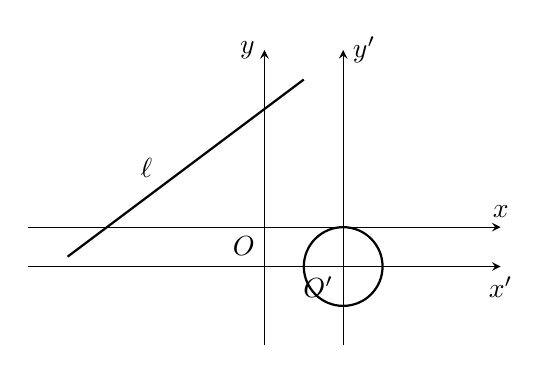
\begin{tikzpicture}[>=stealth, scale=.5]
    \draw[->](-6,0)--(6,0)node[above]{$x$};
\draw[->](-6,-1)--(6,-1)node[below]{$x'$};
\draw[->](0,-3)--(0,4.5)node[left]{$y$};
\draw[->](2,-3)--(2,4.5)node[right]{$y'$};
\draw[thick](2,-1)node[below left=-.1]{$O'$}circle(1);
\node [below left]{$O$};
\draw[domain=-5:1, thick]plot(\x, 3+.75*\x);
\node at (-3,1.5){$\ell$};
\end{tikzpicture}
    \caption{}
\end{figure}
\end{solution}

\subsection*{4.1 练习}
\begin{enumerate}
    \item 把坐标系$xOy$平移到原点$O'$的坐标为$(-3,2)$，得到坐标系$x'O'y'$，试填写下表中同一个点在两个坐标系中相应的坐标：
\begin{center}
\begin{tabular}{c|ccccc}
\hline
在$xOy$平面上  &   $O(0,0)$ &$O'(-3,2)$& $A(3,-4)$& $B(\quad)$& $C(\quad)$\\
\hline
在$x'O'y'$平面上 & $O(\quad )$ & $O'(\quad )$ &$A(\quad)$&$B(-2,1)$&$C(-2,-6)$\\
\hline    
\end{tabular}
\end{center}
\item 点$M$在坐标系$xOy$中的坐标是$(5,-4)$，在坐标系$x'O'y'$中的坐标是$(7,4)$，试求出这个平移变换．
    \item 把坐标系$xOy$平移到原点$O'$的坐标为$(2,-3)$，求曲线
    $x^2+y^2-4x+6y-3=0$在新坐标系中的方程，并画出新坐标轴和曲线.
    \item 试确定一个平移变换，它能把下列圆的方程分别化成${x'}^2+{y'}^2=R^2$的形式：
\begin{multicols}{2}
\begin{enumerate}[(1)]
\item $(x+3)^2+(y-1)^2=1$
\item $(x+2)^2+y^2=4$
\item $x^2+(y+5)^2=25$
\item $x^2+y^2-4x+4y+7=0$   
\end{enumerate}
\end{multicols}
\end{enumerate}

\section{利用移轴化简二元二次方程}
在前一节我们已经看到，适当地平移坐标轴可以化简曲线的方程，本节将研究如何选取新的坐标系，通过移轴来化简方程.

\begin{example}
    用平移变换化简方程
    \begin{equation}
 4x^2+9y^2+8x-36y+4=0       \tag{1}
    \end{equation}
并画出新坐标系和方程的曲线.
\end{example}

\begin{solution}
\textbf{解法1：}（配方法）由(1)，得
\[4(x^2+2x+1)+9(y^2-4y+2^2)=-4+4+36\]

\noindent
\begin{minipage}{.52\textwidth}
即
\[4(x+1)^2+9(y-2)^2=36\]
两边同除以36，得
\begin{equation}
    \frac{(x+1)^2}{3^2}+\frac{(y-2)^2}{2^2}=1  \tag{2}
\end{equation}
令$\begin{cases}
    x+1=x'\\ y-2=y'
\end{cases}$
则(2)变成
\begin{equation}
\frac{{x'}^2}{3^2}+\frac{{y'}^2}{2^2}=1\tag{3}
\end{equation}
\end{minipage}
\hfill
\begin{minipage}{.45\textwidth}
\centering
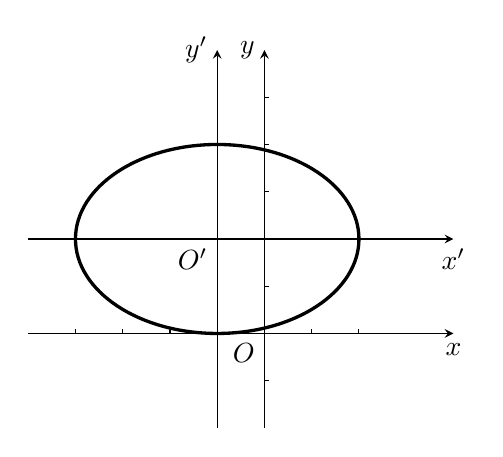
\begin{tikzpicture}[>=stealth, scale=.6]
\draw[->](-4,0)--(5,0)node[below]{$x'$};
\draw[->](0,-4)--(0,4)node[left]{$y'$};
\node[below left]{$O'$};
\draw[->](-4,-2)--(5,-2)node[below]{$x$};
\draw[->](1,-4)--(1,4)node[left]{$y$};
\node at (1,-2)[below left]{$O$};
\draw[very thick](0,0)ellipse (3 and 2);
\foreach \x in {1,2,3}
{
    \draw(\x,-2)--(\x,-2+.1);
    \draw(1,\x)--(1.1,\x);
    \draw(1,-\x)--(1.1,-\x);
    \draw(-\x,-2)--(-\x,-2+.1);
}

\end{tikzpicture}
\captionof{figure}{}
\end{minipage}

在新坐标系$x'O'y'$中，(3)是标准方程．新坐标系和方程的曲线如图4.4所示.

\textbf{解法2：}（待定系数法）

设$\begin{cases}
    x=x'+h\\ y=y'+k
\end{cases}$代入(1)，得
\[4(x'+h)^2+9(y'+k)^2+8(x'+h)-36(y'+k)+4=0\]
即
\begin{equation}
    4{x'}^2+9{y'}^2+(8h+8)x'+(18k-36)y'+(4h^2+9k^2+8h-36k+4)=0 \tag{4}
\end{equation}
令$\begin{cases}
    8h+8=0 \\ 18k-36=0
\end{cases}\Rightarrow \begin{cases}
    h=-1\\ k=2
\end{cases}$
代入(4)，得
\[4{x'}^2+9{y'}^2-36=0\]
即
\[\frac{{x'}^2}{3^2}+\frac{{y'}^2}{2^2}=1\]
（以下略）
\end{solution}

\begin{remark}
    用移轴化简方程，关键是找出新坐标系的原点$O'$在原坐标系下的坐标$(h,k)$. 这里使用的两种方法都是常用的．很明显，解法1的计算量要小些．
\end{remark}

\begin{example}
已知$4x^2-5y^2-16x-10y+31=0$.
\begin{enumerate}[(1)]
\item 用移轴化简这个方程；
\item 画出两个坐标系，并作方程的曲线；
\item 在两个坐标系中分别求出曲线的中心、焦点、准线和渐近线.  
\end{enumerate}
\end{example}

\begin{solution}
\begin{enumerate}[(1)]
    \item 用配方法
\[\begin{split}
    4(x^2-4x+4)-5(y^2+2y+1)&=-31+16-5\\
    4(x-2)^2-5(y+1)^2&=-20
\end{split} \]

\noindent
\begin{minipage}{.5\textwidth}
$\therefore\quad -\frac{(x-2)^2}{5}+\frac{(y+1)^2}{4}=1$

令$\begin{cases}
    x-1=x'\\ y+1=y'
\end{cases}$\hfill (1)

代入上式，得 
\begin{equation}
    -\frac{{x'}^2}{5}+\frac{{y'}^2}{4}=1 \tag{2}
\end{equation}

\item 两个坐标系$xOy$与$x'O'y'$［其中$O'$在$xOy$中的坐标是$(2,-1)$］以及方程的曲线如图4.5所示．
\item 曲线是双曲线，它在两个坐标中有关元素如下：

\end{minipage}
\hfill
\begin{minipage}{.45\textwidth}
\centering
\begin{tikzpicture}[>=stealth, scale=.5]
\draw[->](-5,0)--(5,0)node[below]{$x'$};
\draw[->](0,-6)--(0,6)node[left]{$y'$};
\draw[->](-5,1)--(5,1)node[below]{$x$};
\draw[->](-2,-6)--(-2,6)node[left]{$y$};
\node[below left]{$O'$};
\node at (-2,1)[above left]{$O$};
\draw[domain=-4:4, very thick, smooth, samples=100]plot(\x, {(0.8*\x*\x+4)^(0.5)});
\draw[domain=-4:4, very thick, smooth, samples=100]plot(\x, {-sqrt(0.8*\x*\x+4)});
\draw[domain=-4.5:4.5, thick, smooth]plot(\x, {2/2.236*\x});
\draw[domain=-4.5:4.5, thick, smooth]plot(\x, {-2/2.236*\x});
\tkzDefPoints{0/3/F_1, 0/-3/F_2}
\tkzDrawPoints(F_1,F_2)
\tkzLabelPoints[right](F_1,F_2)
\foreach \x in {-4,-3,-2,...,3}
{
    \draw(\x,1)--(\x,1.2);
    \draw(\x,0)--(\x,0.2);
    \draw(-2,\x)--(-2.2,\x);
    \draw(0,\x)--(-.2,\x);
}

\end{tikzpicture}
\captionof{figure}{}
\end{minipage}

\end{enumerate}

   













\end{solution} 


\begin{center}
\begin{tabular}{c|cccc}
\hline
& 中心 & 焦点& 准线 & 渐近线\\
\hline
在$x'O'y'$中 &  $(0,0)$ &  $\left(0,3\right),\; (0,-3)$ &  $y'=\pm\frac{4}{3}$& $\frac{x'}{\sqrt{5}}\pm\frac{y'}{2}=0$\\
在$xOy$中 &  $\left(2,-1\right)$ &  $\left(2,2\right),\; (2,-4)$ &  $y+1=\pm\frac{4}{3}$& $\frac{x-2}{\sqrt{5}}\pm\frac{y+1}{2}=0$\\
\hline
\end{tabular}
\end{center}



\begin{remark}
\begin{enumerate}
    \item 正确、熟练地使用配方法是解题的基础．否则，配方出错，后面就徒劳了．
    \item 作方程的曲线，是根据(2)，在坐标系$x'O'y'$中画的，这种作法比较简便．
    \item 求曲线的诸元素，先是在坐标系$x'O'y'$中按标准方程(2)进行的，然后只须把$x'$和$y'$分别依据坐标变换公式(1)换成$(x-2)$和$(y+1)$就行了.
\end{enumerate}
\end{remark}

\begin{example}
    证明二次函数$y=ax^2+bx+c\; (a\ne 0)$的图形是一条抛物线，并求其顶点、焦点和准线.
\end{example}

\begin{analyze}
     若能把$y=ax^2+bx+c\; (a\ne 0)$化成抛物线的标准方程就行了.
\end{analyze}

\begin{solution}
   把右边配方，得 
\[y=a\left(x+\frac{b}{2a}\right)^2+\frac{4ac-b^2}{4a}\]
改写成
\begin{equation}
    \left(x+\frac{b}{2a}\right)^2=\frac{1}{a}\left(y-\frac{4ac-b^2}{4a}\right) \tag{1}
\end{equation}
令$\begin{cases}
    x'=x+\frac{b}{2a}\\[1.5ex]
    y'=y-\frac{4ac-b^2}{4a}
\end{cases}$代入(1)，得
\begin{equation}
    {x'}^2=\frac{1}{a}{y'}
\end{equation}

由此可见，二次函数$y=ax^2+bx+c$的图形是以$O'\left(-\frac{b}{2a},\; \frac{4ac-b^2}{4a}\right)$为顶点，对称轴平行于$y$轴的抛物线. 当$a>0$时，开口向上，当$a<0$时，开口向下．如图4.6所示．
\begin{figure}[htp]
    \centering
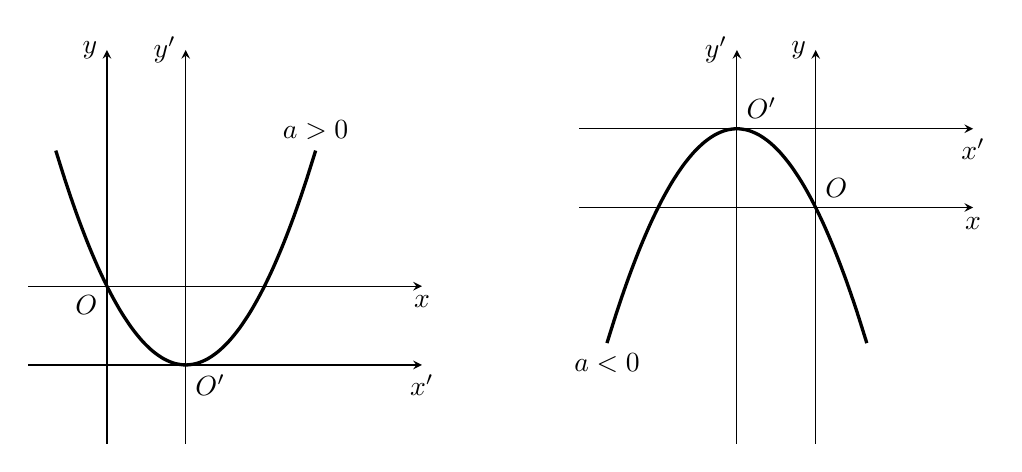
\begin{tikzpicture}[>=stealth]
\begin{scope}
    \draw[->](0,-1)--(0,4)node[left]{$y'$};
    \draw[->](-1,-1)--(-1,4)node[left]{$y$};
\draw[->](-2,0)--(3,0)node[below]{$x'$};
\draw[->](-2,1)--(3,1)node[below]{$x$};
\draw[domain=-1.65:1.65, smooth, very thick]plot(\x, \x*\x)node[above]{$a>0$};
\node at (0,0)[below right]{$O'$};
\node at (-1,1)[below left]{$O$};
\end{scope}
\begin{scope}[xshift=7cm, yshift=3cm]
    \draw[->](0,-4)--(0,1)node[left]{$y'$};
    \draw[->](1,-4)--(1,1)node[left]{$y$};
\draw[->](-2,0)--(3,0)node[below]{$x'$};
\draw[->](-2,-1)--(3,-1)node[below]{$x$};
\draw[domain=1.65:-1.65, smooth, very thick]plot(\x, -\x*\x)node[below]{$a<0$};
\node at (0,0)[above right]{$O'$};
\node at (1,-1)[above right]{$O$};
\end{scope}
\end{tikzpicture}
    \caption{}
\end{figure}

欲求其顶点、焦点和准线，应分两种情况：
\begin{enumerate}[(1)]
    \item 若$a>0$，抛物线开口向上，$2p=\frac{1}{a}\Rightarrow \frac{p}{2}=\frac{1}{4a}$.
\begin{center}
\begin{tabular}{c|ccc}
\hline
& 顶点 & 焦点& 准线\\
\hline
在$x'O'y'$中 &  $(0,0)$ &  $\left(0,\frac{1}{4a}\right)$ &  $y'=-\frac{1}{4a}$\\
在$xOy$中 &  $\left(\frac{-b}{2a},\; \frac{4ac-b^2}{4a}\right)$ &  $\left(\frac{-b}{2a},\; \frac{4ac-b^2+1}{4a}\right)$ &  $y=-\frac{1}{4a}+\frac{4ac-b^2}{4a}$\\
\hline
\end{tabular}
\end{center}

    \item 若$a<0$，抛物线开口向下，$2p=\frac{-1}{a}\Rightarrow \frac{p}{2}=\frac{-1}{4a}$.
\begin{center}
\begin{tabular}{c|ccc}
\hline
& 顶点 & 焦点& 准线\\
\hline
在$x'O'y'$中 &  $(0,0)$ &  $\left(0,\frac{1}{4a}\right)$ &  $y'=-\frac{1}{4a}$\\
在$xOy$中 &  $\left(\frac{-b}{2a},\; \frac{4ac-b^2}{4a}\right)$ &  $\left(\frac{-b}{2a},\; \frac{4ac-b^2+1}{4a}\right)$ &  $y=-\frac{1}{4a}+\frac{4ac-b^2}{4a}$\\
\hline
\end{tabular}
\end{center}
\end{enumerate}
\end{solution}


\subsection*{4.2 练习}
\begin{enumerate}
    \item 平移坐标轴，（用配方法）把下列方程化成标准方程：
\begin{multicols}{2}
  \begin{enumerate}[(1)]
    \item $9x^2+4y^2+36x-8y+4=0$
    \item $x^2-4y^2-4x-24y-16=0$
    \item $y=\frac{1}{4}x^2-x-2$
\end{enumerate}  
\end{multicols}

    \item 平移坐标轴（用待定系数法），把下列方程化成标准方程：
    \begin{multicols}{2}
    \begin{enumerate}[(1)]
        \item $3x^2+2y^2-6y-1=0$
        \item $3x^2-6x+y=0$
        \item $x^2-2y^2-4x+2y-1=0$
    \end{enumerate}    
    \end{multicols}

    \item 平移坐标轴，把方程$x^2-5y^2-8x-10y+16=0$化成标准形式，并写出在老坐标系中曲线的中心、焦点、准线和渐
    近线方程.
    \item  求下列曲线的焦点坐标和对称轴方程：
\begin{multicols}{2}
\begin{enumerate}[(1)]
\item $2x^2+y^2-4x-2y=0$
\item $x^2-2y^2-6x+4y+3=0$
\item $x^2-4x+4y=0$
\end{enumerate}
\end{multicols}

    \item  求适合下列条件的曲线方程：
\begin{enumerate}[(1)]
\item 中心为$O'(-2,1)$，长半轴长为10，焦距为12，焦点在平行于$x$轴的直线上的椭圆；
\item 虚轴的长是8，两顶点是$A(2,1)$和$A'(2,-5)$的双曲线；
\item 焦点是$F(3,-3)$，准线是$y=1$的抛物线.
\end{enumerate}

\end{enumerate}





\chapter{极坐标}

直角坐标系是最常用的一种坐标系，但它并不是用“数对”表示点的位置的唯一的方法. 例如，炮兵指示射击目标，用直角坐标就不方便，通常是指出目标的方位（即方向）和距离. 在航海、航空中也是使用类似的方法. 这种用方向和距离表示点的位置的思想就是下面要讲的极坐标的基本思想.

\section{极坐标系}
在平面内取一个定点$O$，从$O$出发引一条射线$\vv{Ox}$，并取
定长度单位和角度的正方向（通常取逆时针方向）. 这样，平面上就建立了\textbf{极坐标系}. 此时，点$O$称为\textbf{极点}，$\vv{Ox}$称为\textbf{极轴}（图5.1）．对于平面内任意一点$M$，以$\rho$表示有向线段$\vv{OM}$的数量，以$\theta$表示$O$转到$\vv{OM}$的有向角，则\textbf{有序数对}$(\rho,\theta)$可以唯一地确定点
$M$的位置，称为点$M$的\textbf{极坐标}，$\rho$称为\textbf{极径}，
$\theta$称为\textbf{极角}. 建立了极坐标系的平面称为\textbf{极坐标平面}.

\begin{figure}[htp]
    \centering
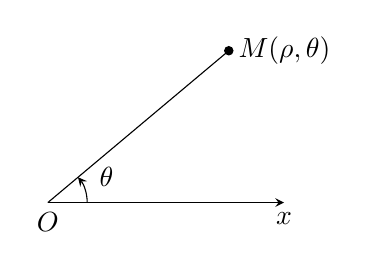
\begin{tikzpicture}[>=stealth]
\draw[->](0,0)--(3,0)node[below]{$x$};
\node[below]{$O$};
\draw(0,0)--(40:3)node[right]{$M(\rho,\theta)$};
\draw[->](.5,0) arc (0:40:.5)node[right=.15cm]{$\theta$};
\draw[fill](40:3)circle(1.5pt);
\end{tikzpicture}    
    \caption{}
\end{figure}

\begin{example}
已知点的极坐标为$A\left(2,\; \frac{3}{4}\pi\right)$、$B\left(3,\; -\frac{3}{4}\pi\right)$、$C\left(4,\; -\frac{\pi}{2}\right)$、$D\left(1,\pi\right)$、$E\left(-2,\; \frac{\pi}{4}\right)$，在极坐标平面上分别找出点的位置.
\end{example}

\begin{solution}
先确定极角$\theta$的终边，再在终边或其反向延长线上找出极径为$\rho$的点的位置（图5.2）．

    对于$E\left(-2,\; \frac{\pi}{4}\right)$，先找出$\theta=\frac{\pi}{4}$的终边$OM$.

$\because\quad \rho=-2$，即有向线段$\vv{OE}$的数量为$-2$

$\therefore\quad $点$E$应在$\vv{OM}$的反向延长线上，且$|OE|=2$.
\end{solution}


\noindent
\begin{minipage}{.48\textwidth}
\centering
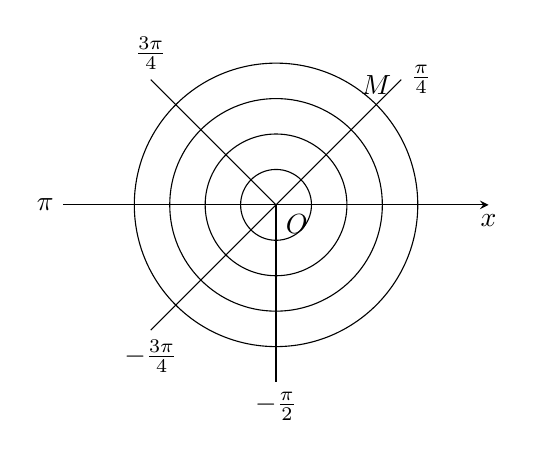
\begin{tikzpicture}[>=stealth, scale=.45]
\draw[->](-6,0)node[left]{$\pi$}--(6,0)node[below]{$x$};
\foreach \x in {1,2,3,4}
{
    \draw(0,0)circle(\x);
}
\node[below right]{$O$};
\draw(0,0)--(0,-5)node[below]{$-\frac{\pi}{2}$};
\draw(0,0)--(90+45:5)node[above]{$\frac{3\pi}{4}$};
\draw(180+45:5)node[below]{$-\frac{3\pi}{4}$}--(45:5)node[right]{$\frac{\pi}{4}$};
\tkzDefPoint(45+90:2){A}
\tkzDefPoint(-45-90:3){B}
\tkzDefPoint(-90:4){C}
\tkzDefPoint(180:1){D}
\tkzDefPoint(-45-90:2){E}
\tkzDrawPoints(A,B,C,D,E)
\tkzDefPoints{0/0/O}
\tkzLabelPoints[right](A)
\tkzLabelPoints[below](D,B,E)
\tkzLabelPoints[below right](C)
\node at (45:4)[above]{$M$};
\end{tikzpicture}
\captionof{figure}{}
\end{minipage}
\hfill
\begin{minipage}{.48\textwidth}
\centering
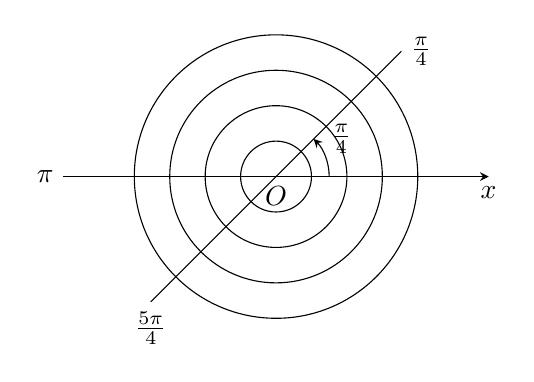
\begin{tikzpicture}[>=stealth, scale=.45]
\draw[->](-6,0)node[left]{$\pi$}--(6,0)node[below]{$x$};
\foreach \x in {1,2,3,4}
{
    \draw(0,0)circle(\x);
}
\node[below]{$O$};
\draw(180+45:5)node[below]{$\frac{5\pi}{4}$}--(45:5)node[right]{$\frac{\pi}{4}$};
\tkzDefPoint(45:4){A}
\tkzDefPoint(-3,0){B}
\tkzDrawPoints(A,B)
\tkzDefPoints{0/0/O}
\tkzLabelPoints[right](A)
\tkzLabelPoints[below](B)
\draw[->](1.5,0) arc (0:45:1.5)node[right=.1cm]{$\frac{\pi}{4}$};

\end{tikzpicture}
\captionof{figure}{}
\end{minipage}

\begin{example}
    在极坐标平面上，已知点$A$、$B$、$O$的位置如图5.3，分别写出它们的极坐标.
\end{example}

\begin{solution}
点$A$的极坐标可以是$\left(4,\; \frac{\pi}{4}\right)$，也可以是$\left(4,\; \frac{\pi}{4}+2k\pi\right)$，其中$k\in\Z$，还可以是$\left(-4,\; \frac{\pi}{4}+\pi\right)$, 或者$\left(-4,\; \frac{\pi}{4}+\pi+2k\pi\right)$，其中$k\in\Z$.

同样，点$B$的极坐标可以是$(3,\pi+2k\pi)$，其中$k\in\Z$, 也可以是$(-3,0+2k\pi)$，其中$k\in\Z$.

极点$O$的极径为零，极角可以取任意实数$\alpha$，即$O(0,\alpha)$，其中$\alpha\in\R$.

概括上面的例子可知，给定极坐标$(\rho,\theta)$以后，在极坐标平面上有且只有一个点与之对应；反过来，在极坐标平面上，给定一个点以后，若$(\rho,\theta)$是该点的极坐标，则$(\rho,\theta+2k\pi)$
与$(-\rho,\theta+\pi+2k\pi)$，其中$k\in\Z$，都是该点的极坐标. 这就是所谓，\textbf{点的极坐标的多值性}. 这一点和直角坐标系的情况是不同的. 但是，根据需要，如果对$\rho$、$\theta$作一些限制，如限定$\rho\ge 0$, $0\le \theta<2\pi$，那么除极点外，平面内的点和它的极坐标就可以一一对应了.
\end{solution}

\subsection*{5.1 练习}
\begin{enumerate}
\item 口答：图中$A$、$B$、$C$、$D$、$E$、$F$、$G$、$H$、$O$各点的极坐标$(\rho>0,\quad 0\le \theta<2\pi)$.
\item 在极坐标平面上作出下列各点：
\begin{enumerate}[(1)]
    \item $A\left(2,\;\frac{\pi}{6}\right),\; B(6,-120^{\circ}),\; C(0,5^{\circ}),\; D\left(3,\;-\frac{\pi}{4}\right),\; E(4,0),\; F(2,270^{\circ})$
    \item $A\left(4,\;\frac{\pi}{3}\right),\; B\left(4,\frac{\pi}{2}\right),\; C(4,\pi),\; D\left(4,\;\frac{4\pi}{3}\right),\;  E\left(4,\;\frac{11\pi}{6}\right)$，并说明这五个点有什么关系？
    \item $A\left(5,\;\frac{\pi}{3}\right),\; B\left(-2,\;\frac{\pi}{3}\right),\; C\left(3,\;\frac{4\pi}{3}\right),\; D\left(0,\;\frac{\pi}{3}\right),\; E\left(-3,\frac{4}{3}\pi\right)$，并说明这五个点有什么关系？
\end{enumerate}

\begin{figure}[htp]
    \centering
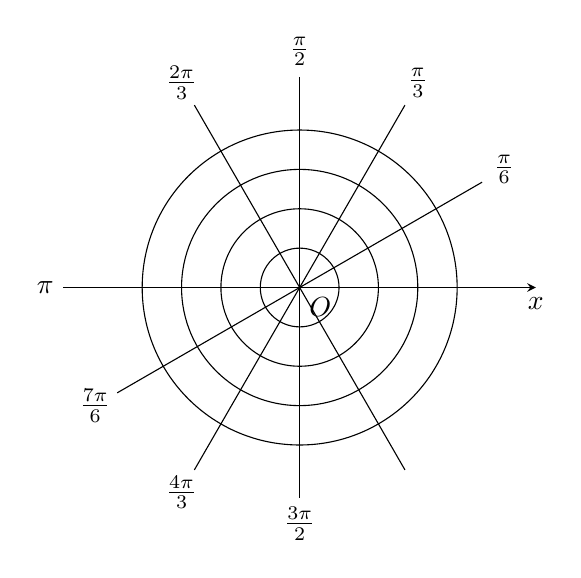
\begin{tikzpicture}[>=stealth, scale=.5]
\draw[->](-6,0)node[left]{$\pi$}--(6,0)node[below]{$x$};
\foreach \x in {1,2,3,4}
{
    \draw(0,0)circle(\x);
}

\foreach \x in {30,60,90,120}
{
    \draw(\x:5.35)--(\x+180:5.35);
}
\node at (30:6){$\frac{\pi}{6}$};
\node at (60:6){$\frac{\pi}{3}$};
\node at (120:6){$\frac{2\pi}{3}$};
\node at (90:6){$\frac{\pi}{2}$};
\node at (-90:6){$\frac{3\pi}{2}$};
\node at (30+180:6){$\frac{7\pi}{6}$};
\node at (60+180:6){$\frac{4\pi}{3}$};
\tkzDefPoints{0/4/C, -4/0/E, 3/0/H, 0/-2/G}
\tkzDefPoint(120:3){D}
\tkzDefPoint(60:2){B}
\tkzDefPoint(30:4){A}
\tkzDefPoint(-120:3){F}
\tkzDrawPoints(A,B,C,D,E,F,G,H)
\tkzLabelPoints[above right](B,C)
\tkzLabelPoints[below right](F,G,H)
\tkzLabelPoints[below left](E)
\tkzLabelPoints[above](A,D)

\node[below right]{$O$};


\end{tikzpicture}
    \caption*{第1题}
\end{figure}


\item 在极坐标平面上，分别作出下列各题中的两个点，并说明这两点间有什么关系：
\begin{multicols}{2}
\begin{enumerate}[(1)]
    \item $\left(3,\;\frac{\pi}{6}\right),\quad \left(3,\;\frac{5\pi}{6}\right)$
    \item $\left(2,\;\frac{\pi}{3}\right),\quad \left(2,\;-\frac{\pi}{3}\right)$
    \item $\left(5,\;\frac{4\pi}{3}\right),\quad \left(5,\;\frac{5\pi}{3}\right)$
    \item $\left(2,\; -\pi\right),\quad \left(2,\; \pi\right)$
    \item $\left(-2,\;\frac{5\pi}{3}\right),\quad \left(-3,\;\frac{2\pi}{3}\right)$
    \item $\left(-5,\;-\frac{\pi}{3}\right),\quad \left(-5,\;\frac{\pi}{3}\right)$
\end{enumerate}
\end{multicols}
\end{enumerate}

\section{曲线的极坐标方程}

在直角坐标系中，曲线与方程定义的本质是：曲线上的点集和方程的实数解集之间通过点的直角坐标建立了一一对应的关系. 在极坐标系中，关键在于能否使曲线$C$上的点集和方程$F(\rho,\theta)=0$的实数解集之间通过点的极坐标建立一一对应的关系.

\begin{figure}[htp]
    \centering
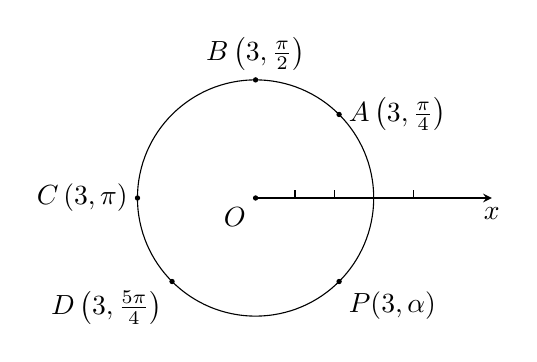
\begin{tikzpicture}[>=stealth, scale=.5]
    \draw[->](0,0)--(6,0)node[below]{$x$};
\draw(0,0)node[below left]{$O$} circle(3);
\draw[fill](0,0) circle(1.5pt);
\draw[fill](45:3)node[right]{$A\left(3,\frac{\pi}{4}\right)$} circle(1.5pt);
\draw[fill](90:3)node[above]{$B\left(3,\frac{\pi}{2}\right)$} circle(1.5pt);
\draw[fill](180:3)node[left]{$C\left(3,\pi\right)$} circle(1.5pt);
\draw[fill](-135:3)node[ below left]{$D\left(3,\frac{5\pi}{4}\right)$} circle(1.5pt);
\draw[fill](-45:3)node[ below right]{$P(3,\alpha)$} circle(1.5pt);
\foreach \x in {1,2,3,4}
{
    \draw(\x,0)--(\x,.2);
}


\end{tikzpicture}
    \caption{}
\end{figure}


\textbf{实例：}
 对于以极点$O$为圆心，以3为半径的圆（图5.4）和极坐标方程$\rho=3$：任取圆上一个点$P$，其极坐标总能写成形式$(3,\alpha)$，这里$\alpha\in\R$，有序数对$(3,\alpha)$显然是方程$\rho=3$的解；反过来，方程$\rho=3$的任一解$(3,\theta_0)$，其中$\theta_0\in\R$，对应的点显然也都在这个圆上. 这说明，上述一一对应关系可以通过点的极坐标建立起来，因此，把方程$\rho=3$看作是上述圆的代数形式是合乎情理的.但是必须指出，在极坐标系中由于点的极坐标的多值性，有时会产生麻烦.例如，点$D\left(3,\frac{5\pi}{4}\right)$的极坐标若写成$\left(-3,\frac{\pi}{4}\right)$时，有序数对$\left(-3,\frac{\pi}{4}\right)$就不是$\rho=3$的解. 这是和直角坐标系不同的地方.

 基于以上分析，在极坐标系中有

 \begin{thm}
 {定义} 在极坐标平面上，如果曲线$C$和方程$F(\rho,\theta)=0$满足：
 \begin{enumerate}[(1)]
 \item 曲线上的每一个点\textbf{至少}能写出它的一个极坐标，该极坐标是方程的一个解；
 \item 以方程的每一个实数解为极坐标的点都在曲线上．那么，$F(\rho,\theta)=0$就称为\textbf{曲线$C$的极坐标方程}，$C$就称为\textbf{方程$F(\rho,\theta)=0$的曲线}.     
 \end{enumerate}
 \end{thm}

 求曲线的极坐标方程的方法和步骤同求直角坐标方程类似，即把曲线看作满足某种特征性质（几何性质）的点的集合或轨迹，然后设法把这一特征性质转化成代数形式.

\subsection{直线的极坐标方程}
 平面上两个独立条件确定一条直线，两个条件的不同给法将导出不同形式的极坐标方程.

 对于直线$\ell$，由极点$O$向$\ell$引垂线$OD$（图5.5），极轴$\vv{Ox}$转到$\vv{OD}$的角记为$\omega\; (0\le \omega<2\pi)$叫做法相角，垂线的长
$|OD|$（就是极点到$\ell$的距离），记为$p\; (p\ge 0)$. 显然，$\omega$、$p$确定以后，直线$\ell$应是唯一的.

\noindent
\begin{minipage}{.45\textwidth}
    \centering
\begin{tikzpicture}[>=stealth]
\draw[->](0,0)node[below]{$O$}--(4,0)node[below]{$x$};
\tkzDefPoints{0/0/O, 3/0/A, 1.5/2.5/B}
\tkzDrawLines[add = 0.3 and 0](A,B)
\node at (B)[right]{$\ell$};
\tkzDefPointBy[projection = onto A--B](O) \tkzGetPoint{D}
\draw[dashed](O)--node[left]{$p$}(D);
\tkzLabelPoints[right](D)
\tkzMarkRightAngles[size=.15](O,D,A)
\tkzMarkAngles[mark=none, size=.5, ->](A,O,D)
\tkzLabelAngle[pos=.8](A,O,D){$\omega$};
\end{tikzpicture}
\captionof{figure}{}
\end{minipage}
\hfill
\begin{minipage}{.45\textwidth}
\centering
\begin{tikzpicture}[>=stealth]
\draw[->](0,0)node[below]{$O$}--(4,0)node[below]{$x$};
\tkzDefPoints{0/0/O, 3/0/A, 1.5/2.5/P}
\tkzDrawLines[add = 0.25 and 0.2](A,P)
\node at (P)[right]{$P(\rho,\theta)$};
\draw(O)--node[left]{$\rho$}(P);

\tkzDefPointBy[projection = onto A--P](O) \tkzGetPoint{D}
\draw[dashed](O)--node[right=.5cm]{$p$}(D);
\tkzLabelPoints[right](D)
\tkzMarkRightAngles[size=.15](O,D,A)
\tkzMarkAngles[mark=none, size=.5, ->](A,O,D)
\tkzLabelAngle[pos=.8](A,O,D){$\omega$};

\tkzMarkAngles[mark=none, size=1.2, ->](A,O,P)
\tkzLabelAngle[pos=1.5](A,O,P){$\theta$};
\node at (3.5,-.5)[below]{$\ell$};




\end{tikzpicture}
\captionof{figure}{}
\end{minipage}


\begin{example}
    如图5.6，已知直线$\ell$，$OD\bot \ell$，交$\ell$于$D$，$\angle xOD=\omega$, $|OD|=p$，求$\ell$的极坐标方程.
\end{example}

\begin{solution}
    在$\ell$上取动点$P(\rho,\theta)$. 连$OP$，则$|OP|=\rho$, $\angle xOP=\theta$. 显然，诸条件可以都集中到${\rm Rt}\triangle DOP$中：
\[|OP|\cdot \cos\angle DOP=|OD|\]
即
\begin{equation}
    \rho\cos(\theta-\omega)=p  \tag{1}
\end{equation}
\end{solution}

\begin{rmk}
\begin{enumerate}
\item 若把动点$P(\rho,\theta)$取在点$D$的下方，不会影响结论(1)，
\item (1)式的结构特征：$\rho$与$\theta-\omega$的余弦乘积为常数.
\end{enumerate}
\end{rmk}

方程(1)称为\textbf{直线方程的一般式}. 对于(1)，研究几个特例是有趣的.
\begin{enumerate}[(1)]
    \item 令$\rho=0$（这是过极点的直线），由方程(1)得
\[\rho\cos(\theta-\omega)=0\]
\[\rho=0\quad \text{或}\quad \cos(\theta-\omega)=0 \Rightarrow\theta=\omega+\frac{\pi}{2}\; (\rho\in\R)\]
由于$\rho=0$包含在后者之中，所以上式等价于
\begin{equation}
    \theta=\omega+\frac{\pi}{2}\quad (\rho\in\R) \tag{1}
\end{equation}

\item 当$p\ne 0$时（直线不过极点），让$\omega$分别取特殊值$0,\; \frac{\pi}{2},\; \pi,\; \frac{3\pi}{2}$，这时(1)变为
\begin{equation}
\begin{split}
    \rho\cos\theta=p,&\qquad  \rho\sin\theta=p\\
    \rho\cos\theta=-p,&\qquad  \rho\sin\theta=-p\\
\end{split}\tag{2}
\end{equation}
对于上述四种情况，请读者分别画出直线的图形.
\end{enumerate}

\begin{rmk}
    对于(1)，我们特别强调$\rho\in\R$（若只取$\rho\ge 0$就仅仅表示从极点发出的一条射线，而不代表整条直线$\ell$）.
\end{rmk}

\begin{thm}{思考题}
方程$\rho\sin\left(\theta-\frac{\pi}{3}\right)=4$是否表示直线？为什么，请画出其图形.
\end{thm}

\begin{example}
    已知直线$\ell$的倾角为$\alpha$，且过$P_1(\rho_1,\theta_1)$，求$\ell$的方程（图5.7）．
\end{example}

\begin{analyze}
     设动点为$P(\rho,\theta)$. 容易看出，诸条件集中于$\triangle P_1OP$是可行的.
\end{analyze}

\begin{solution}
\[|OP|=\rho,\quad  |OP_1|=\rho_1,\quad  \angle OPP_1=\alpha-\theta,\quad \beta=\pi-(\alpha-\theta_1)\]
    在$\triangle P_1OP$中，由正弦定理，得
\[\frac{\rho}{\sin[\pi-(\alpha-\theta_1)]}=\frac{\rho_1}{\sin(\alpha-\theta)}\quad \Rightarrow\quad \rho=\frac{\rho_1\sin(\alpha-\theta_1)}{\sin(\alpha-\theta)}\]
\end{solution}


\noindent
\begin{minipage}{.45\textwidth}
    \centering
\begin{tikzpicture}[>=stealth]
\draw[->](0,0)node[below]{$O$}--(4,0)node[below]{$x$};
\tkzDefPoints{0/0/O, 2/0/A, 2.5/2.5/P, 4/0/B}
\tkzDrawLines[add = 0.3 and 0.3](A,P)
\tkzDefMidPoint(A,P) \tkzGetPoint{P1}
\draw[dashed](O)--node[right=.2cm]{$\rho_1$}(P1);
\draw(O)--node[left]{$\rho$}(P);
\tkzMarkAngles[mark=none, size=.5, ->](A,O,P)
\tkzLabelAngle[pos=.7](A,O,P){$\theta$}
\tkzMarkAngles[mark=none, size=1, ->](A,O,P1)
\tkzLabelAngle[pos=1.2](A,O,P1){$\theta_1$}
\tkzMarkAngles[mark=none, size=.5, ->](B,A,P)
\tkzLabelAngle[pos=.8](B,A,P){$\alpha$}
\tkzMarkAngles[mark=none, size=.3, ->](P,P1,O)
\tkzLabelAngle[pos=.5](P,P1,O){$\beta$}
\node at (P)[right]{$P(\rho,\theta)$};
\node at (P1)[right]{$P_1(\rho_1,\theta_1)$};
\end{tikzpicture}
\captionof{figure}{}
\end{minipage}
\hfill
\begin{minipage}{.45\textwidth}
\centering
\begin{tikzpicture}[>=stealth]
\draw[->](0,0)node[below]{$O$}--(4,0)node[below]{$x$};
\tkzDefPoints{0/0/O, 2/0/A, 1.5/1.2/P1}
\tkzDrawLines[add = 1.2 and 1.2](A,P1)

\tkzDefPointWith[linear, K=1.7](A,P1)   \tkzGetPoint{P}
\tkzDefPointWith[linear, K=2](P1,A)   \tkzGetPoint{P2}
\tkzDrawSegments(O,P)
\tkzDrawSegments[dashed](O,P1 O,P2)

\node at (P)[right]{$P(\rho,\theta)$};
\node at (P1)[right]{$P_1(\rho_1,\theta_1)$};
\node at (P2)[right]{$P_2(\rho_2,\theta_2)$};

\draw(O)--node[left]{$\rho$}(P);
\draw[dashed](O)--node[above]{$\rho_1$}(P1);
\draw[dashed](O)--node[below]{$\rho_2$}(P2);


\tkzMarkAngles[mark=none, size=1, ->](A,O,P1)
\tkzLabelAngle[pos=1.2](A,O,P1){$\theta_1$}

\tkzMarkAngles[mark=none, size=.5, ->](A,O,P)
\tkzLabelAngle[pos=.7](A,O,P){$\theta$}

\tkzMarkAngles[mark=none, size=.7, <-](P2,O,A)
\tkzLabelAngle[pos=1](P2,O,A){$\theta_2$}


\end{tikzpicture}
\captionof{figure}{}
\end{minipage}

\begin{example}
    已知直线$\ell$过$P_1(\rho_1,\theta_1)$, $P_2(\rho_2,\theta_2)$两个点，求$\ell$的方程（图5.8).
\end{example}

\begin{analyze}
   设动点为$P(\rho,\theta)$，则$\triangle P_1OP$, $\triangle P_1OP_2$与$\triangle P_2OP$都是知道两边及夹角，从而面积可以表示出来.
\end{analyze}

\begin{solution}
\[\begin{split}
\because\quad \angle P_1OP=\theta-\theta_1\quad &\Rightarrow\quad  S_1=\frac{1}{2}\rho\rho_1\sin(\theta-\theta_1)\\
\angle P_2OP_1=\theta_1-\theta_2\quad &\Rightarrow\quad  S_2=\frac{1}{2}\rho_1\rho_2\sin(\theta_1-\theta_2)\\
\angle P_2OP=\theta-\theta_2\quad &\Rightarrow\quad  S=\frac{1}{2}\rho\rho_2\sin(\theta-\theta_2)\\
\end{split}\]
很明显$S=S_1+S_2$

$\therefore\quad \frac{1}{2}\rho\rho_1\sin(\theta-\theta_1)+\frac{1}{2}\rho_1\rho_2\sin(\theta_1-\theta_2)=\frac{1}{2}\rho\rho_2\sin(\theta-\theta_2)$
\begin{equation}
    \frac{\sin(\theta-\theta_1)}{\rho_2}+\frac{\sin(\theta_1-\theta_2)}{\rho}=\frac{\sin(\theta-\theta_2)}{\rho_1}  \tag{2}
\end{equation}
\end{solution}

\subsection{圆的极坐标方程}

\begin{example}
    试求以$C(\rho_0,\theta_0)$为圆心，以$r$为半径的圆的极坐标方程（图5.9）．
\end{example}


\noindent
\begin{minipage}{.6\textwidth}\CTEXindent
    \begin{solution}
        $\triangle COP$的三边为$\rho_0,\rho,r$，$\angle COP=\theta-\theta_0$
        
        利用余弦定理，得
        \[r^2=\rho^2+\rho^2_0-2\rho\rho_0\cos(\theta-\theta_0)\]
        即
        \begin{equation}
           \rho^2-2\rho\rho_0\cos(\theta-\theta_0)+\rho^2_0-r^2=0 \tag{3}
        \end{equation}
        (3)称为\textbf{圆方程的一般式}.
        \end{solution}
\end{minipage}
\hfill
\begin{minipage}{.38\textwidth}
\centering
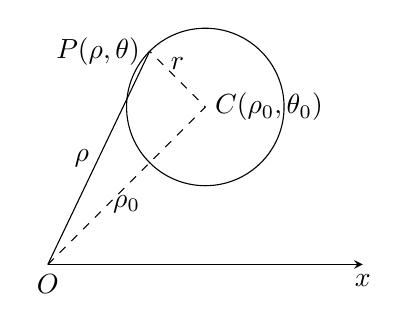
\begin{tikzpicture}[>=stealth]
    \draw[->](0,0)node[below]{$O$}--(4,0)node[below]{$x$};    
    \draw(2,2)node[right]{$C(\rho_0,\theta_0)$} circle (1);
    \draw[dashed](0,0)--node[below]{$\rho_0$}(2,2)--node[above]{$r$}+(90+45:1)node[left]{$P(\rho,\theta)$};
    \draw(0,0)--node[left]{$\rho$}(2-1.414/2,2+1.414/2);
    
    \end{tikzpicture}
\captionof{figure}{}
\end{minipage}

我们也来研究一下(3)的特例：
\begin{enumerate}
    \item 当$\rho_0=0$时（圆心在极点的圆），由(3)得
\begin{equation}
    \rho =r\quad (\theta\in\R) \tag{4}    
\end{equation}
    \item 当$\rho_0=r$时（这是过极点的圆），由(4)得
\begin{equation}
    \rho^2-2\rho r\cos(\theta-\theta_0)=0  \tag{*}    
\end{equation}
$\therefore\quad \rho=0$或$\rho-2r\cos(\theta-\theta_0)=0$.


由于$\rho=0$也包含在后者之中，所以(*)等价于
\begin{equation}
\rho=2r\cos(\theta-\theta_0)  \tag{5}
\end{equation}
在(5)中令$\theta_0$分别取$0,\; \frac{\pi}{2},\; \pi,\; \frac{3\pi}{2}$时得到
\begin{equation}
    \begin{split}
        \rho=2r\cos\theta,&\qquad  \rho=2r\sin\theta\\
        \rho=-2r\cos\theta,&\qquad  \rho=-2r\sin\theta\\
    \end{split}\tag{2}
    \end{equation}
对于上述四种情况，请读者分别画出它们的图形.
\end{enumerate}

\noindent
\begin{minipage}{.47\textwidth}\CTEXindent
\begin{example}
    已知锐角$\angle AOB=2\alpha$内有一个动点$P$, $PM\bot OA$于$M$，$PN\bot OB$于$N$，且四边形$PMON$的面积为常数$C^2$，以$O$为极点，$\angle AOB$的平分线$Ox$为极轴，求动点$P$的轨迹的极坐标方程（图5.10）.
\end{example}


\begin{analyze}
    设动点$P$为$(\rho,\theta)$. 四边形$PMON$被$OP$分割成两个直角三角形. 这两个三角形的面积都可以表出.
\end{analyze}

\end{minipage}
\hfill
\begin{minipage}{.5\textwidth}
\centering
\begin{tikzpicture}[>=stealth]
\draw(0,0)node[below left]{$O$}--(5,0)node[below]{$B$};
\tkzDefPoints{0/0/O, 3/3/P}
\tkzDefPoint(60:5){A}
\tkzDefPoint(30:6){x}
\tkzDefPointBy[projection =  onto A--O](P)   \tkzGetPoint{M}
\tkzDefPointBy[projection = onto B--O](P)  \tkzGetPoint{N}
\tkzDrawSegments(A,O P,M P,N)
\draw(O)--node[above]{$\rho$}(P); 
\tkzDrawSegments[->](O,x)
\tkzLabelPoints[below](x,N)
\tkzLabelPoints[left](M)
\tkzLabelPoints[right](A)
\node at (P)[right]{$P(\rho,\theta)$};
\tkzMarkRightAngles[size=.2](P,M,O P,N,O)

\tkzMarkAngles[mark=none, size=.6, ->](B,O,x)
\tkzLabelAngle[pos=.8](B,O,x){$\alpha$};

\tkzMarkAngles[mark=none, size=1, ->](x,O,P)
\tkzLabelAngle[pos=1.2](x,O,P){$\theta$};

\tkzMarkAngles[mark=none, size=1.6, ->](x,O,A)
\tkzLabelAngle[pos=1.8](x,O,A){$\alpha$};

\end{tikzpicture}
\captionof{figure}{}
\end{minipage}

\begin{solution}
$\because\quad \angle POA=\alpha-\theta,\quad |OM|=\rho\cos(\alpha-\theta),\quad |PM|=\rho\sin(\alpha-\theta)$

$\therefore\quad S_{POM}=\frac{1}{2}|OM|\cdot |PM|=\frac{1}{2}\rho^2\cos(\alpha-\theta)\sin (\alpha-\theta)=\frac{1}{4}\rho^2 \sin (2\alpha-2\theta)$

又$\because\quad \angle NOP=\alpha+\theta,\quad |ON|=\rho\cos(\alpha+\theta),\quad |PN|=\rho\sin(\alpha+\theta)$

$\therefore\quad S_{PNO}=\frac{1}{2}|ON|\cdot |PN|=\frac{1}{2}\rho^2\cos(\alpha+\theta)\sin (\alpha+\theta)=\frac{1}{4}\rho^2\sin (2\alpha+2\theta)$

又$\therefore\quad $已知四边形$ONPM$的面积为$C^2$，
而
\[\text{四边形$ONPM$的面积}=S_{POM}+S_{PNO}\]
$\therefore\quad C^2=\frac{1}{4}\rho^2 \sin(2\alpha-2\theta)+\frac{1}{4}\rho^2\sin(2\alpha+2\theta)$
即
\[\rho^2\sin(2\alpha-2\theta)+\rho^2\sin(2\alpha+2\theta)=4C^2\]

\subsection{三种圆锥曲线的极坐标方程}

在第三章里我们已经看到，抛物线、椭圆、双曲线可以统一定义为：到定点$F$（焦点）与定直线$\ell$（准线）距离之比等于常数$e$的点的轨迹，当$e=1$时是抛物线，当$0<e<1$时是椭圆，当$e>1$时是双曲线.

本节将依照这个统一定义，求出三种圆锥曲线的统一的极坐标方程，并做初步地应用.

\noindent
\begin{minipage}{.5\textwidth}
\CTEXindent
    过点$F$作准线$\ell$的垂线，垂足为$K$，以焦点$F$为极点，以$FK$的反向延长线$\vv{Fx}$为极轴，建立极坐标系（图5.11).

    设$|KF|=p$，曲线上的动点为$M(\rho,\theta)$，连$MF$，则$|MF|=\rho$，作$MA\bot\ell$于$A$，则
    \[\frac{|MF|}{|MA|}=e\]
\end{minipage}
\hfill
\begin{minipage}{.45\textwidth}
\centering
\begin{tikzpicture}[>=stealth]
\draw[->](-1,0)--(4,0)node[below]{$x$};
\draw(0,-2)node[right]{$\ell$}--(0,2);
\node[below left]{$K$};
\draw[domain=-1.5:1.5, very thick, smooth]plot({\x*\x+1},\x);
\tkzDefPoints{2.5625/1.25/M, 2.5625/0/B, 0/1.25/A, 5/0/x, 1.5/0/F, 0/2/y}
\tkzDrawSegments(M,A M,B)
\tkzDrawLine[add=0 and .5](F,M)
\tkzLabelPoints[left](A)
\tkzLabelPoints[below](B)
\node at (M)[below right]{$M(\rho,\theta)$};
\node at (F)[below]{$F(O)$};
\tkzMarkRightAngles[size=.15](M,A,y M,B,x)
\draw(F)--node[above]{$\rho$}(M);

\tkzMarkAngles[mark=none, size=.4, ->](x,F,M)
\tkzLabelAngle[pos=.6](x,F,M){$\theta$};

\end{tikzpicture}
\captionof{figure}{}
\end{minipage}

过$M$作$MB\bot Fx$于$B$，则
\[|MA|=|BK|=|KF|+|FB|=p+\rho\cos\theta\]
代入上式，得
\begin{equation}
\frac{\rho}{p+\rho\cos\theta}=e\quad \Rightarrow\quad \rho=\frac{ep}{1-e\cos\theta} \tag{6}
\end{equation}
(6)就是上述三种圆锥曲线的统一的极坐标方程，其中，$\rho,\theta$是动点坐标；$p$是焦准距，它是描写曲线位置特征的参数；$e$是离心率，它是描写曲线形状特征的参数.

\noindent
\begin{minipage}{.48\textwidth}
\centering
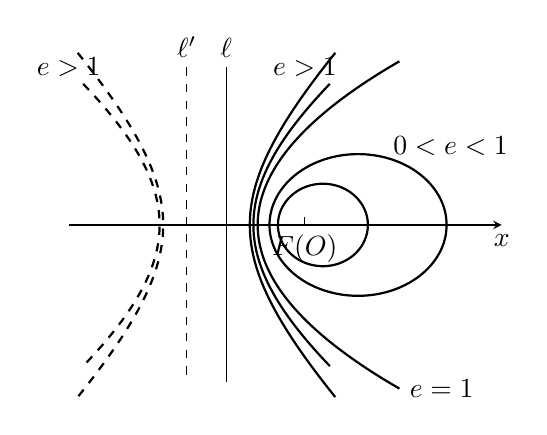
\begin{tikzpicture}[>=stealth]
\draw[->](-3,0)--(2.5,0)node[below]{$x$};


\foreach \e  in {.4,.6  }
{
    \draw[domain=0:360, samples=100, thick, smooth]plot({\e*1.2/(1-\e*cos(\x))*cos(\x)}, {\e*1.2/(1-\e*cos(\x))*sin(\x)});
}



\foreach \e  in {1}
{
    \draw[domain=180-120:180+120, samples=100, thick, smooth]plot({\e*1.2/(1-\e*cos(\x))*cos(\x)}, {\e*1.2/(1-\e*cos(\x))*sin(\x)})node[right]{$e=1$};
}
\foreach \e in {1.4,1.2}
{
    \draw[domain=180-100:180+100, samples=100, thick, smooth]plot({\e*1.2/(1-\e*cos(\x))*cos(\x)}, {\e*1.2/(1-\e*cos(\x))*sin(\x)});
    \draw[domain=180-100:180+100, samples=100, thick, dashed, smooth]plot({-\e*1.2/(1-\e*cos(\x))*cos(\x)-2.5}, {\e*1.2/(1-\e*cos(\x))*sin(\x)});
}
\draw(-1,2)node[above]{$\ell$}--(-1,-2);
\draw[dashed](-1.5,2)node[above]{$\ell'$}--(-1.5,-2);
\node at (1,1)[right]{$0<e<1$};
\node at (0,2)[]{$e>1$};
\node at (-3,2)[]{$e>1$};
\draw(0,0)node[below]{$F(O)$}--(0,.1);
\end{tikzpicture}
\captionof{figure}{}
\end{minipage}
\hfill
\begin{minipage}{.48\textwidth}
\centering
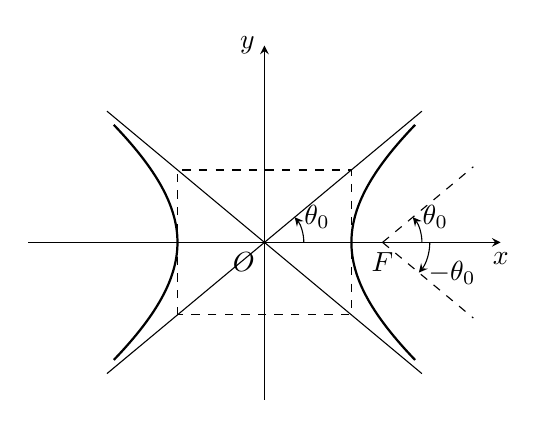
\begin{tikzpicture}[>=stealth]
\draw[->](-3,0)--(3,0)node[below]{$x$};
\draw[->](0,-2)--(0,2.5)node[left]{$y$};
\node[below left]{$O$};

\foreach \e  in {1.2}
{
    \draw[domain=180-100:180+100, samples=100, thick, smooth]plot({\e*1/(1-\e*cos(\x))*cos(\x)+1.65}, {\e*1/(1-\e*cos(\x))*sin(\x)});
    \draw[domain=180-100:180+100, samples=100, thick, smooth]plot({-\e*1/(1-\e*cos(\x))*cos(\x)-1.65}, {\e*1/(1-\e*cos(\x))*sin(\x)});
}
\draw[domain=-2:2, smooth]plot(\x, {1/1.2*\x});
\draw[domain=-2:2, smooth]plot(\x, {-1/1.2*\x});

\draw[dashed](-1.1,-.92) rectangle (1.1,.92);
\draw[->](.5,0) arc (0:39.8:.5)node[right]{$\theta_0$};
\draw[dashed](1.5,0)node[below]{$F$}--+(39.8:1.5);
\draw[dashed](1.5,0)--+(-39.8:1.5);

\draw[->](2,0) arc (0:39.8:.5)node[right]{$\theta_0$};
\draw[->](2+.1,0) arc (0:-39.8:.6)node[right]{$-\theta_0$};


\end{tikzpicture}
\captionof{figure}{}
\end{minipage}



当$e\in(0,1)$，(6)表示椭圆，若$\theta$从0变到$2\pi\; (0\le \theta<2\pi)$，就得到椭圆上全部的点（图5.12）．

当$e=1$时，(6)表示抛物线，若$\theta$从0变到$2\pi\; (0<\theta<2\pi)$，就得到抛物线上所有的点；

当$e\in(1,+\infty)$时，(6)表示双曲线. 我们知道，双曲线的渐近线的倾角若记为$\theta_0$与$\pi-\theta_0$，则$\cos\theta_0=\frac{a}{c}=\frac{1}{e}$. 由此，若$\theta$从$\theta_0$变到$2\pi-\theta_0$，就得到双曲线右支上所有的点；若$\theta$从$-\theta_0$到$\theta_0$，此时$\rho$取负值，就能得到双曲线左支上所有的点（图5.13）．应
注意在图5.12中，$F$是双曲线的右焦点，椭圆的左焦点，$\ell$是双曲线的右准线，椭圆的左准线.

\end{solution}

\noindent
\begin{minipage}{.65\textwidth}
\begin{example}
已知抛物线的方程是$\rho=\frac{p}{1-\cos\theta}$
（图5.14），
\begin{enumerate}[(1)]
\item 试求其过焦弦$AB$的弦长；
\item 证明：在过焦弦中以通径为最短；
\item 试求过焦弦$AB$中点的轨迹方程．
\end{enumerate}
\end{example}

\begin{analyze}
由于$AB$是过焦弦，若点$A$的极坐标是$(\rho_1,\theta_1)$，那么点$B$的极坐标就可以写成$(\rho_2,\theta_1+\pi)$，则$|AB|=\rho_1+\rho_2$.  
\end{analyze}
\end{minipage}
\hfill
\begin{minipage}{.3\textwidth}
\centering
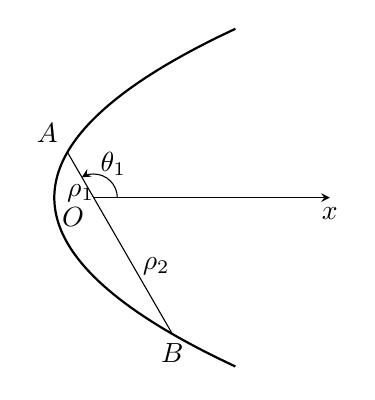
\begin{tikzpicture}[>=stealth]
\draw[->](0,0)node[below left]{$O$}--(3,0)node[below]{$x$};
\draw[domain=180-130:180+130, samples=100, thick, smooth]plot({1/(1-cos(\x))*cos(\x)}, {1/(1-cos(\x))*sin(\x)});
\draw(120:2/3)node[above left]{$A$}--node[below]{$\rho_1$}(0,0)--node[right]{$\rho_2$}(-60:2)node[below]{$B$};
\draw[->](.3,0)arc (0:120:.3);
\node at (60:.5){$\theta_1$};
\end{tikzpicture}
\captionof{figure}{}
\end{minipage}

\begin{solution}
\begin{enumerate}[(1)]
    \item 设$A(\rho_1,\theta_1)$, $B(\rho_2,\theta_1+\pi)$. 则
\[\rho_1=\frac{p}{1-\cos\theta_1},\quad \rho_2=\frac{p}{1-\cos(\theta_1+\pi)}=\frac{p}{1+\cos\theta_1}\]
\[|AB|=\rho_1+\rho_2=\frac{p}{1-\cos\theta_1}+\frac{p}{1+\cos\theta_1}=\frac{2p}{\sin^2\theta_1}\]

    \item 当$\theta=\frac{\pi}{2}$时，弦$AB$就是通径.
    
$\therefore\quad $通径的长$=\frac{2p}{\sin^2\frac{\pi}{2}}=2p\le \frac{2p}{\sin^2\theta}=|AB|$

即：过焦弦中以通径为最短.
\item 设弦$AB$的中点为$P(\rho,\theta_1)$. 把弦$AB$所在的直线看作是直线坐标系，点$O$看作原点. 若点$A$的直线坐标记为$(\rho_1)$，则点$B$的直线坐标就应为$(-\rho_2)$. 那么，$A$、$B$的中点$P$的直线坐标就是
\[\rho=\frac{\rho_1+(-\rho_2)}{2}\]

$\therefore\quad \rho=\frac{\frac{p}{1-\cos\theta_1}-\frac{p}{1+\cos\theta_1}}{2}=\frac{2p\cos\theta_1}{2\sin^2\theta_1}=\frac{p\cos\theta_1}{\sin^2\theta_1}$

这就是点$P$轨迹的极坐标方程.
\end{enumerate}
    
\end{solution}

\begin{rmk}
从此例可以看出，对于过焦弦问题，用方程(6)处理是非常简便的. 实际上(6)中的$\rho$就是焦半径.  
\end{rmk}

\begin{example}
    求椭圆$\rho=\frac{16}{5-3\cos\theta}$的长轴和短轴的长.
\end{example}

\begin{solution}
\textbf{解法1：}由方程可得$\rho=\frac{\frac{16}{5}}{1-\frac{3}{5}\cos\theta}$
\[\begin{cases}
    e=\frac{3}{5}\\[1.5ex]
    ep=\frac{16}{5}
\end{cases}\Rightarrow\begin{cases}
    e=\frac{3}{5}\\[1.5ex]
    p=\frac{16}{3}
\end{cases}\Rightarrow\begin{cases}
    \frac{c}{a}=\frac{3}{5}\\[1.5ex]
    \frac{b^2}{c}=\frac{16}{3}\\[1.5ex]
    a^2=b^2+c^2
\end{cases}\Rightarrow\begin{cases}
    c=3\\a=5\\b=4
\end{cases}\]
$\therefore\quad $长轴长$=2a=10$，短轴长$=2b=8$.    

\noindent
\begin{minipage}{.53\textwidth}
\CTEXindent
\textbf{解法2：}在图5.15中
\[\begin{split}
    \rho_1&=\frac{16}{5-3\cos 0}=\frac{16}{2}=8,\quad (\theta=0)\\
    \rho_2&=\frac{16}{5-3\cos\pi}=\frac{16}{8}=2,\quad (\theta=\pi)
\end{split}\]
\end{minipage}
\hfill
\begin{minipage}{.45\textwidth}
\centering
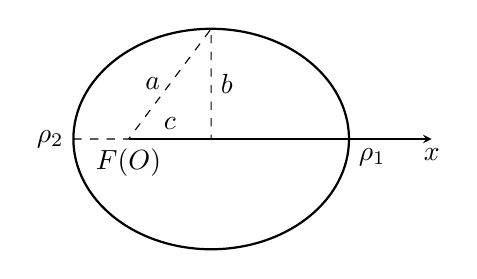
\begin{tikzpicture}[>=stealth, scale=.35]
\draw[->](-3,0)--(8,0)node[below]{$x$};
\draw[thick](0,0) ellipse (5 and 4);
\node at (-3,0)[below]{$F(O)$};
\draw[dashed](-5,0)node[left]{$\rho_2$}--(-3,0)--node[left]{$a$}(0,4)--node[right]{$b$}(0,0)--node[above]{$c$}(-3,0);
\node at (5,0)[below right]{$\rho_1$};



\end{tikzpicture}
\captionof{figure}{}
\end{minipage}

$\therefore\quad $长轴长$=\rho_1+\rho_2=8+2=10$

对椭圆来说，$\frac{\rho_1-\rho_2}{2}=c\quad \Rightarrow\quad c=\frac{8-2}{2}=3$，

而$a^2=b^2+c^2,\quad 2a=10,\quad a=5$

$\therefore\quad b=\sqrt{a^2-c^2}=\sqrt{25-9}=4$

$\therefore\quad$短轴长$=2b=8$

\end{solution}

\subsection*{5.2 练习}
\begin{enumerate}
    \item 求适合下列条件的直线的极坐标方程，并画出图形：
\begin{multicols}{2}
    \begin{enumerate}[(1)]
    \item 过极点，倾角为$\frac{\pi}{4}$
    \item 过点$(4,0)$，且和极轴垂直；
    \item 法向角$\omega=\frac{2\pi}{3}$，且到极点的距离$\rho=2$;
    \item 过点$\left(2,-\frac{\pi}{2}\right)$，且平行于极轴；
    \item 过点$\left(2,\frac{\pi}{3}\right)$，且倾角为$\frac{\pi}{4}$.  
    \end{enumerate}    
\end{multicols}


    \item 作出下列方程的曲线：
\begin{multicols}{2}
 \begin{enumerate}[(1)]
    \item $\rho\cos\left(\theta+\frac{\pi}{3}\right)=2$;
    \item $\rho\sin\left(\theta-\frac{\pi}{4}\right)=1$;
    \item $\rho\sin\theta+\rho\cos\theta=\sqrt{2}$.
\end{enumerate}   
\end{multicols}

    \item 求适合下列条件的圆的极坐标方程，并画图：
\begin{multicols}{2}
\begin{enumerate}[(1)]
    \item 圆心在极点，$r=3$
    \item   圆心在$(2,\pi)$，$r=2$
    \item  圆心在$\left(-3,-\frac{\pi}{2}\right)$, $r=3$
    \item  圆心在$(-2,0)$, $r=1$
    \item  圆心在$(a,0)$, $r=a\; (a>0)$
\end{enumerate}
\end{multicols}

 \item \begin{enumerate}[(1)]
     \item 试求椭圆$\rho=\frac{5}{3-2\cos\theta}$的顶点坐标、焦点坐标和准线方程（在极坐标系中）；
     \item  试求抛物线$\rho=\frac{4}{1-\cos\theta}$的通径的长；
     \item  试求双曲线$\rho=\frac{6}{1-3\cos\theta}$的实轴的长；
      \item  试求椭圆$\rho=\frac{8}{5-3\cos\theta}$中倾角为$\frac{\pi}{3}$的过焦弦的长.
  \end{enumerate}    

\item \begin{enumerate}[(1)]
    \item 利用方程$\rho=\frac{ep}{1-e\cos\theta}$研究椭圆上哪个点离左焦点最远？最近？
    \item 在$\rho=\frac{ep}{1-e\cos\theta}$中，若令$\theta=\frac{\pi}{2}$，则得$\rho=ep$，试解释其几何意义.
\end{enumerate}
\item  说明下列两条直线的位置关系：
\begin{enumerate}[(1)]
    \item $\theta=\alpha$和$\rho\cos(\theta-\alpha)=m\; (m>0)$;
    \item $\theta=\alpha$和$\rho\sin(\theta-\alpha)=n\; (n>0)$.
\end{enumerate}

\item  求出圆$\rho=5\sqrt{3}\cos\theta+5\sin\theta$的圆心和半径.
\item  $F$是焦点，圆锥曲线的方程是$\rho=\frac{ep}{1-e\cos\theta}$, $PQ$是过点$F$的任意弦，证明：
$\frac{1}{|FP|}+\frac{1}{|FQ|}$是一个定值.
\item  若$F$是椭圆$\rho=\frac{ep}{1-e\cos\theta}$的左焦点，弦$PQ$、$RS$相交于$F$，且$PQ\bot RS$，求证
\[\frac{1}{|PQ|}+\frac{1}{|RS|}=\frac{2-e^2}{2ep}\]
\item  从极点$O$作直线和曲线$\rho\cos\theta=4$相交于$M$点，在$OM$上取一点$P$，使$OM\cdot OP=12$，求点$P$的轨迹方程.
\end{enumerate}

\section{极坐标与直角坐标的互化}
极坐标系和直角坐标系是平面上两种不同的坐标系. 平面上同一个点可以有极坐标，也可以有直角坐标，同一条曲线可以有极坐标方程，也可以有直角坐标方程. 为了研究问题方便，有时需要把这两种坐标方程互化. 这个互化的基础就是点的极坐标和直角坐标的互化.

假定平面上这两个坐标系有如下的关系（图5.16）：
\begin{enumerate}[(i)]
    \item 极点与原点重合；
    \item 极轴与$x$轴的正半轴重合；
    \item 单位长相同.
\end{enumerate}

\noindent
\begin{minipage}{.45\textwidth}
\centering
\begin{tikzpicture}[>=stealth]
\draw[->](-2.5,0)--(2,0)node[below]{$x$};
\draw[->](0,-1)--(0,2.5)node[left]{$y$};
\node[below left]{$O$};
\draw[thick](0,0)--node[above]{$\rho$}(130:2.5)node[left]{$M$};
\draw[dashed](130:2.5)--node[left]{$y$}(-1.61,0)node[below]{$x$};
\draw[->](.3,0) arc (0:130:.3);
\node at (65:.5){$\theta$};

\end{tikzpicture}
\captionof{figure}{}
\end{minipage}
\hfill
\begin{minipage}{.45\textwidth}
\centering
\begin{tikzpicture}[>=stealth]
\draw[->](-2,0)--(2.5,0)node[below]{$x$};
\draw[->](0,-2)--(0,2)node[left]{$y$};
\node[below left]{$O$};
\draw[dashed](120:2)--(0,0);
\draw[](-60:2)--(0,0);
\draw[->](.3,0) arc (0:120:.3);
\node at (60:.5){$\theta$};
\draw[fill](-60:1.5)node[right]{$M(\rho,\theta)$}circle(1.5pt);


\end{tikzpicture}
\captionof{figure}{}
\end{minipage}


在这三条前提下，我们来探求点的两种坐标的互化公式. 设$M$是平面上的任一点，它的直角坐标是$(x,y)$，极坐标是$(\rho,\theta)$.当$\rho>0$时，根据任意角三角函数的定义，得
\begin{align}
\begin{cases}
    \frac{x}{\rho}=\cos\theta\\[1.5ex]
    \frac{y}{\rho}=\sin\theta\\
\end{cases}&\Rightarrow  \begin{cases}
    x=\rho\cos\theta\\
    y=\rho\sin\theta\\
\end{cases}\tag{1}\\
&\Rightarrow  \begin{cases}
    \rho^2=x^2+y^2\\
    \tan\theta=\frac{y}{x}& (x\ne 0)\\
\end{cases}\tag{2}
\end{align}

当$\rho<0$时（图5.17），可将点$M(x,y)$
的极坐标$(\rho,\theta)$改写成$(-\rho,\theta+\pi)$，此时$(-\rho)>0$，有
\[\begin{cases}
    \frac{x}{-\rho}=\cos(\theta+\pi)\\[1.5ex]
    \frac{y}{-\rho}=\sin(\theta+\pi)\\
\end{cases}\Rightarrow  \begin{cases}
    x=\rho\cos\theta\\
    y=\rho\sin\theta\\
\end{cases}\]
可见(1)仍然成立，当$\rho=0$时也然. 从而对一切$\rho\in\R$，(1)式都成立.

\begin{example}
    把下列点的极坐标化成直角坐标\footnote{应该指出：直角坐标与极坐标的互化都是在上述三条前提之下进行.}：
\begin{multicols}{2}
\begin{enumerate}[(1)]
    \item $A\left(-8,\; -\frac{\pi}{6}\right)$
    \item $B\left(-2,\; -\frac{\pi}{2}\right)$
\end{enumerate}
\end{multicols}
\end{example}

\begin{solution}
\begin{enumerate}[(1)]
    \item 由公式(1)，得
\[\begin{cases}
    x=(-8)\cos\left(-\frac{\pi}{6}\right)=(-8)\cdot \frac{\sqrt{3}}{2}=-4\sqrt{3}\\[1.5ex]
    y=(-8)\sin\left(-\frac{\pi}{6}\right)=(-8)\cdot \left(\frac{1}{2}\right)=4
\end{cases}\]
$\therefore\quad A\left(-4\sqrt{3},4\right)$
    \item 由公式(1)，得
\[\begin{cases}
    x=(-2)\cos\left(-\frac{\pi}{2}\right)=0\\[1.5ex]
    y=(-2)\sin\left(-\frac{\pi}{2}\right)=2
\end{cases}\]
$\therefore\quad B\left(0,2\right)$
\end{enumerate}
\end{solution}

\begin{example}
    把下列点的直角坐标化成极坐标：
\begin{multicols}{3}
\begin{enumerate}[(1)]
    \item $P(0,-4)$
    \item $Q(-3,3)$
    \item $N(-5,-2)$
\end{enumerate}
\end{multicols}
\end{example}


\noindent
\begin{minipage}{.55\textwidth}
\begin{solution}
在坐标系中，先画出这三个点（图5.18）．从图上可以看出：
\begin{enumerate}[(1)]
\item 点$P(0,-4)$的极坐标是$\left(4,\frac{3\pi}{2}\right)$，或者写成$\left(-4,\frac{\pi}{2}\right)$;
\item 点$Q(-3,3)$的极坐标是$\left(3\sqrt{2},\;\frac{3\pi}{4}\right)$;
\item 点$N(-5,-2)$的极坐标是$$\left(\sqrt{29},\;\pi+\arctan \frac{2}{5}\right)$$当然，写成$\left(-\sqrt{29},\;\arctan\frac{2}{5}\right)$也行.
\end{enumerate}
\end{solution}
\end{minipage}
\hfill
\begin{minipage}{.43\textwidth}
\centering
\begin{tikzpicture}[>=stealth, scale=.5]
\draw[->](-6,0)--(4,0)node[below]{$x$};
\draw[->](0,-5)--(0,5)node[left]{$y$};
\node[below right]{$O$};
\tkzDefPoints{-3/3/Q, -5/-2/N, 0/-4/P, 0/0/O}
\tkzDrawPoints(P,Q,N)
\tkzDrawSegments(O,P O,Q O,N)
\draw[dashed](-5,0)--(-5,-2)node[below]{$N(-5,-2)$}--(0,-2);
\node at (Q)[above]{$Q(-3,3)$};
\node at (P)[right]{$P(0,-4)$};
\draw[->](.75,0) arc (0:180+21.8:.75);
\node at (90:1)[right]{$\pi+\arctan\frac{2}{5}$};

\foreach \x in {1,2,3,4}
{
    \draw(-\x,0)--(-\x,.2);
    \draw(0,\x)--(.2,\x);
    \draw(0,-\x)--(.2,-\x);
}
\end{tikzpicture}
\captionof{figure}{}
\end{minipage}


由以上两例概括出点的极坐标与直角坐标系的互化方法是
\begin{equation}
P(\rho,\theta)\xrightleftharpoons[\text{用图示法}]{\text{用公式(1)}} P(x,y)  \tag{*}
\end{equation}


\begin{example}
    化下列直角坐标方程为极坐标方程：
\begin{multicols}{3}
\begin{enumerate}[(1)]
    \item $x^2+y^2-2ax=0$;
    \item $x-\sqrt{3}y=0$;
    \item $y^2=2px\; (p>0)$.
\end{enumerate}
\end{multicols}
\end{example}

\begin{solution}
    把公式(1)代入直角坐标方程，化简即可.
\begin{enumerate}[(1)]
    \item $\rho^2-2a\rho\cos\theta=0\quad \Rightarrow\quad \rho(\rho-2a\cos\theta)=0$
\[\rho=0\quad \text{或}\quad \rho=2a\cos\theta\]

$\because\quad \rho=0$包含在$\rho=2a\cos\theta$之中

$\therefore\quad $原式的极坐标方程是$\rho=2a\cos\theta$.

    \item $\rho \cos\theta-\sqrt{3}\rho\sin\theta=0\quad \Rightarrow\quad \rho\left(\cos\theta-\sqrt{3}\sin\theta\right)=0$
    \[\rho=0\quad \text{或}\quad \tan\theta=\frac{1}{\sqrt{3}}\Rightarrow \theta=\frac{\theta}{6}\; (\rho\in\R)\]


$\because\quad \rho=0$包含在$\theta=\frac{\theta}{6}\; (\rho\in\R)$之中

$\therefore\quad $原式的极坐标方程是$\theta=\frac{\theta}{6}\; (\rho\in\R)$.

    \item $(\rho\cos\theta)^2=2p(\rho\cos\theta)\quad \Rightarrow\quad \rho(\rho\sin^2\theta-2p\cos\theta)=0$
\[\rho=0\quad \text{或}\quad \rho\sin^2\theta-2p\cos\theta=0\]
\begin{equation}
    \rho=\frac{2p\cos\theta}{\sin^2\theta}\quad (\sin\theta\ne 0) \tag{3}
\end{equation}

$\because\quad \rho=0$包含在(3)之中

$\therefore\quad $原式的极坐标方程是(3).
\end{enumerate}
\end{solution}

\begin{thm}
{思考题} 在例5.12（3）中抛物线$y^2=2px\; (p>0)$的极坐标方程为什么不是$p=\frac{p}{1-\cos\theta}$而是(3)呢？
\end{thm}


\begin{example}
    化下列极坐标方程为直角坐标方程：
\begin{multicols}{2}
\begin{enumerate}[(1)]
    \item $\rho=5\sin\theta$
    \item $\rho^2=a^2\sin2\theta$
    \item $\rho=\frac{ep}{1-e\cos\theta}$
\end{enumerate}
\end{multicols}
\end{example}

\begin{solution}
若以公式(2)代入，运算较繁. 不如先作如下变形，再以(1)代入：
\begin{enumerate}[(1)]
\item $\rho=5\sin\theta$，以$\rho$乘两边，得
\[\rho^2=5\rho\sin\theta\]
注意：这样做，方程增了一个解$\rho=0$, 但显见它适合（1），

$\therefore\quad $是同解变形．

$\therefore\quad x^2+y^2=5y$
\item $\rho^2=a^2\sin2\theta$以$\rho^2$乘两边，得
\[\rho^4=a^2\cdot 2p\rho \sin\theta\cdot \rho\cos\theta\]

注意：这样做，方程增了一个二重解$\rho=0$，但它也适合（2），

$\therefore\quad $仍为同解变形．

$\therefore\quad (x^2+y^2)^2=2a^2xy$.
\item $\rho=\frac{ep}{1-e\cos\theta}\quad \Rightarrow\quad \rho-e\rho\cos\theta=ep$
\[\begin{split}
 & \Rightarrow\quad    \sqrt{x^2+y^2}=ex+ep\\
 & \Rightarrow\quad     x^2+y^2=e^2 x^2+2e^2xp+e^2p^2\\
 & \Rightarrow\quad     (1-e^2)x^2+y^2-2e^2 px-e^2 p^2=0
\end{split} \]
\end{enumerate}
\end{solution}

从以上两例概括出极坐标方程与直角坐标方程互化的方法是
\begin{equation}
    \varphi(\rho,\theta)=0 \xrightleftharpoons[\text{用公式(1)}]{\text{凑出}\rho\cos\theta,\; \rho\sin\theta} f(x,y)=0 \tag{**}
\end{equation}

以下研究几个应用两种坐标（方程）互化的例子.



    \begin{example}
        若${\rm Rt}\triangle ACB$的直角四等分线交斜边于$P_1$、$P_2$、$P_3$（图5.19），试求$\frac{1}{OP_1}+\frac{1}{OP_2}+\frac{1}{OP_3}$的值（已知$CA=a$, $CB=b$）
    \end{example}
    
\begin{analyze}
$OP_1$、$OP_2$、$OP_3$是直线$AB$上的三个点$P_1$、$P_2$、$P_3$到$O$点的距离. 而且$OP_1$、$OP_2$、$OP_3$与直线$CA$的夹角分别是$\frac{\pi}{8},\; \frac{\pi}{4},\; \frac{3\pi}{8}$. 若以$C$为极点，
$CA$所在直线为极轴，建立极坐标系，那么$OP_1$、$OP_2$、$OP_3$就可用极径表示出来.
\end{analyze}

\begin{solution}
    如图5.19建立极坐标系．由于$AO=a$, $BO=b$，直线$AB$的直角坐标方程为
\[\frac{x}{a}+\frac{y}{b}=1\xRightarrow[]{\text{用公式(1)}} \frac{1}{\rho}=\frac{\cos\theta}{a}+\frac{\sin\theta}{b}\]

\noindent
\begin{minipage}{.52\textwidth}
    于是
    \[\begin{split}
    \frac{1}{|OP_1|}&=\frac{1}{\rho_1}=\frac{\cos\frac{\pi}{8}}{a}+\frac{\sin\frac{\pi}{8}}{b}\\
    \frac{1}{|OP_2|}&=\frac{1}{\rho_2}=\frac{\cos\frac{\pi}{4}}{a}+\frac{\sin\frac{\pi}{4}}{b}\\
    \frac{1}{|OP_3|}&=\frac{1}{\rho_3}=\frac{\cos\frac{3\pi}{8}}{a}+\frac{\sin\frac{3\pi}{8}}{b}\\
    \end{split}\]
\end{minipage}
\hfill
\begin{minipage}{.45\textwidth}
\centering
\begin{tikzpicture}[>=stealth, scale=1.2]
    \draw[->](0,0)node[below left]{$C(O)$}--(2.5,0)node[below]{$x$};
    \draw (0,0)--(0,2.5)node[above]{$B$};
    \tkzDefPoints{0/0/O, 0/2.5/B, 2/0/A}
    
    \foreach \x in {1,2,3}
    {
        \tkzDefPoint(45/2*\x:1){P\x}
        \tkzInterLL(O,P\x)(A,B) \tkzGetPoint{P_\x}
        \tkzLabelPoints[right](P_\x)
        \tkzDrawSegments(O,P_\x)
    }
    \tkzDrawPolygon(A,O,B)
    \tkzLabelPoints[below](A)
    \tkzMarkAngles[mark=none, size=.8](A,O,P_1 P_2,O,P_3)
    \tkzMarkAngles[mark=none, size=.7](P_1,O,P_2 P_3,O,B)
    \tkzLabelAngle[pos=1](A,O,P_1){$\tfrac{\pi}{8}$}
    
\end{tikzpicture}
\captionof{figure}{}
\end{minipage}


\[\begin{split}
    \text{原式}&=\frac{1}{a}\left(\cos\frac{\pi}{8}+\cos\frac{\pi}{4}+\cos\frac{3\pi}{8}\right)+\frac{1}{b}\left(\sin\frac{\pi}{8}+\sin\frac{\pi}{4}+\sin\frac{3\pi}{8}\right)\\
    &=\frac{1}{a}\cdot \frac{\sqrt{2}}{2}\left(1+2\cos\frac{\pi}{8}\right)+\frac{1}{b}\cdot \frac{\sqrt{2}}{2}\left(1+2\cos\frac{\pi}{8}\right)\\
    &=\frac{\sqrt{2}(a+b)}{2ab}\left(1+2\cos\frac{\pi}{8}\right)
\end{split}\]
\end{solution}

\begin{remark}
    此题如此简捷地解出，关键是“想到”把$OP_1$、$OP_2$、$OP_3$看成极径，从而需要把直线$AB$表成极坐标方程.
\end{remark}

\begin{example}
    试求曲线$\rho\cos\theta=-2$与曲线$\rho+6\cot\theta\cdot \csc\theta=0$的交点.
\end{example}

\begin{analyze}
     对这两个方程，特别是后者，不易识别，若消元去解三角方程也不易，先化成直角坐标方程试试看.
\end{analyze}

\begin{solution}
$\rho\cos\theta=-2\quad \Rightarrow\quad x=-2$\hfill （原来这是直线！）
\begin{align}
    \rho+6\cot\theta\cdot \csc\theta=0 \quad &\Rightarrow\quad \rho+\frac{6\cos\theta}{\sin\theta}\cdot \frac{1}{\sin\theta}=0 \tag{\text{显然$\sin\theta\ne 0$}}\\
    \quad &\Rightarrow\quad \rho\sin^2\theta+6\cos\theta=0 \tag{\text{$\rho=0$显然是其解}}\\
    \quad &\Rightarrow\quad \rho^2\sin^2\theta +6\rho\cos\theta=0\nonumber\\
    \quad &\Rightarrow\quad y^2=-6x \tag{\text{原来这是抛物线！}}
\end{align}
\[\begin{cases}
    x=-2\\ y^2=-6x
\end{cases}\Rightarrow\quad \begin{cases}
    x=-2\\ y=\pm 2\sqrt{3}
\end{cases}\]

$\therefore\quad $所求交点的直角坐标是$\left(-2,2\sqrt{3}\right)$和$\left(-2,-2\sqrt{3}\right)$，极坐标是
$\left(4,\frac{2\pi}{3}\right)$和$\left(4,\frac{4\pi}{3}\right)$.
\end{solution}

这两例告诉我们：由极坐标方程给出的问题，若不好处
理，就直角坐标化；由直角坐标方程给出的问题，若用极坐标方法处理较简便，就极坐标化. 一句话，\textbf{互化为的是寻求最简方法}.

\subsection*{5.3 练习}
\begin{enumerate}
    \item 已知各点的极坐标为$\left(4,\frac{\pi}{4}\right)$、$\left(2,\frac{4\pi}{3}\right)$、$\left(-7,\pi\right)$、$\left(5,\frac{\pi}{2}\right)$、$\left(-2,-\frac{\pi}{6}\right)$、$\left(-3,-\frac{\pi}{2}\right)$. 写出它们的直角坐标.
    \item 已知各点的直角坐标为$(3,0)$、$(0,2)$、$(3,3)$、$(-3,0)$、$(-2,-3)$、$(0,-4)$、$(3,-4)$、$(0,0)$．
写出它们的极坐标（限制$0\le \theta<2\pi$）.
    \item 化下列极坐标方程为直角坐标方程：
\begin{multicols}{2}
\begin{enumerate}[(1)]
    \item $\rho=5$
    \item $\theta=\frac{\pi}{3}\quad (\rho\in\R)$
    \item $\rho=2\cos\theta$
    \item $\rho^2\cos2\theta=16$
    \item $\rho=a\csc\theta$
    \item $\rho=a^2\sin4\theta$
    \item $\rho^2=64\sin2\theta$
    \item $\rho-3\cot\theta\cdot \csc\theta=0$
    \item $\rho^2=\tan\theta$
    \item $\rho=a\cos2\theta\quad (a>0)$
    \item $\rho^2-2a\rho\cos\theta+a^2-r^2=0$
    \item $\rho=\frac{ep}{1-e\cos\theta}$
\end{enumerate}
\end{multicols}
\item 化下列直角坐标方程为极坐标方程：
\begin{multicols}{2}
\begin{enumerate}[(1)]
    \item $x=7$
    \item $y=-2$
    \item $3x-4y=2$
    \item $xy=4$
    \item $x^2-y^2=a^2$
    \item $x\cos\alpha+y\sin\alpha-p=0$
    \item $(x^2+y^2)^2=a(x^3-3xy^2)$ 
    
    $(a>0)$
\end{enumerate}
\end{multicols}

\item 正三角形的各个顶点在抛物线$y^2=2x$上，其中一个顶点和抛物线顶点重合.求其余两个顶点的坐标.
\item 若$A$、$B$、$C$是椭圆上任取的三个点，且满足关系$\angle AOB=\angle BOC=\angle COA$（$O$是椭圆的中心）. 试证$\frac{1}{|OA|^2}+\frac{1}{|OB|^2}+\frac{1}{|OC|^2}$为定值.

（你能想出几种证法吗？哪一种是最佳解法？）
\item 在抛物线$y^2=4x$上有一个点$A(4,4)$，试在其上找一个点$B$，使$\angle AOB=75^{\circ}$，并求$|AB|$.
\item 把方程$\rho=-\cos^2\theta$化成$(x^2+y^2)^{3/2}=-x^2$是错误的，简述理由，并加以改正.

\end{enumerate}

\section{曲线极坐标方程的应用}

\noindent
\begin{minipage}{.55\textwidth}
\begin{example}
    设点$M$在圆锥曲线
\begin{equation}
    \rho=\frac{ep}{1-e\cos\theta} \tag{1}
\end{equation}
上运动，试求线段$OM$上一点$P$的轨迹，使
$\frac{OP}{PM}=\frac{1}{2}$（图5.20）
\end{example}

\begin{analyze}
    这是一个相关点轨迹问题. 主动点$M$在(1)上运动，求被动点$P$的轨迹.
\end{analyze}
\end{minipage}
\hfill
\begin{minipage}{.42\textwidth}
\centering
\begin{tikzpicture}[>=stealth, scale=1.2]
\draw[->](0,0)--(3.5,0)node[below]{$x$};
\node[below right]{$O(F)$};
\draw[domain=-1.25:1.25, thick, smooth]plot({2*\x*\x-.5}, \x);
\tkzDefPoints{0/0/O, 1.5/1/M, .5/.333/P}
\tkzDrawPoints(O,P,M)
\tkzDrawSegments(O,M)
\node at (P)[right]{$P(\rho,\theta)$};
\node at (M)[above]{$M(\rho_1,\theta_1)$};


\end{tikzpicture}
\captionof{figure}{}
\end{minipage}


\begin{solution}
设动点坐标$P(\rho,\theta)$、$M(\rho_1,\theta_1)$
，由$\frac{OP}{PM}=\frac{1}{2}$可得
\begin{equation}
\begin{cases}
    \frac{\rho}{\rho_1-\rho}=\frac{1}{2}\\[1.5ex]
    \theta=\theta_1
\end{cases}\Rightarrow \begin{cases}
    \rho=\frac{1}{3}\rho_1\\
    \theta=\theta_1
\end{cases}\Rightarrow \begin{cases}
    \rho_1=3\rho \\
    \theta_1=\theta
\end{cases}\tag{2}
\end{equation}
    利用点$M(\rho_1,\theta_1)$在曲线(1)上运动，可得
\begin{equation}
    \rho_1=\frac{ep}{1-e\cos\theta_1} \tag{3}
\end{equation}
(2)代入(3)，得
\begin{equation}
    3\rho=\frac{ep}{1-e\cos\theta} \quad \Rightarrow\quad \rho=\frac{ep}{3-3\cos\theta} \tag{4}
\end{equation}
它是以点$O(F)$为极点，开口向右的抛物线.
\end{solution}

\begin{remark}
这是一个典型的求轨迹的问题. 抓住本质可做推广如下：
\begin{enumerate}[(1)]
\item 点$M$不一定限制在曲线(1)上运动，它可以在任何一条已知极坐标方程的曲线上运动（这是对曲线(1)的推广）；
\item 点$P$不一定限制以$\lambda=\frac{1}{2}$内分$OM$，只要能得出$\rho_1=f(\rho)$就可解（这是对极径关系的推广）；
\item 不一定限制$\theta=\theta_1$，而只要有关系
$\begin{cases}
    \rho_1=\rho\\ \theta_1=\varphi(\theta)
\end{cases}$就可解（这是对极角关系的推广）
\end{enumerate}

如，令$\begin{cases}
    \rho=\rho_1\\
    \theta=\theta_1+\frac{\pi}{2}
\end{cases} \xRightarrow[]{\text{代入(3)}} \rho=\frac{ep}{1-e\sin\theta}  $（图5.21(1)）\hfill (5)

又如，令$\begin{cases}
    \rho=\rho_1\\
    \theta=\theta_1+\pi
\end{cases} \xRightarrow[]{\text{代入(3)}} \rho=\frac{ep}{1+e\cos\theta}  $（图5.21(2)）\hfill (6)

再如，令$\begin{cases}
    \rho=\rho_1\\
    \theta=\theta_1+\frac{3}{2}\pi
\end{cases} \xRightarrow[]{\text{代入(3)}} \rho=\frac{ep}{1+e\sin\theta}  $（图5.21(3)）\hfill (7)
\end{remark}

\begin{figure}[htp]
    \centering
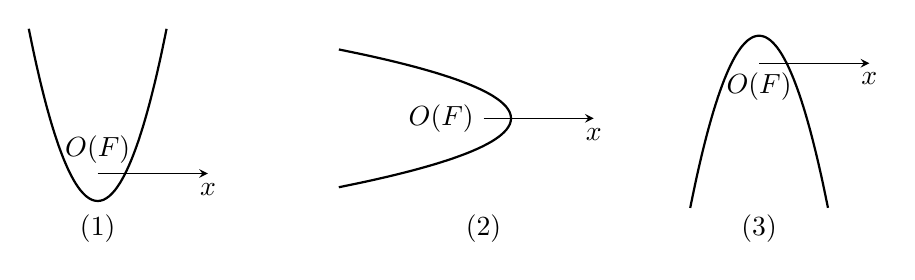
\begin{tikzpicture}[>=stealth, scale=.7]
\begin{scope}
    \draw[->](0,0)--(2,0)node[below]{$x$};
\node[above]{$O(F)$};
\draw[domain=-1.25:1.25, thick, smooth]plot(\x, {2*\x*\x-.5});
\node at (0,-1){(1)};
\tkzDrawPoint(0,0)
\end{scope}
\begin{scope}[xshift=7cm, yshift=1cm]
    \draw[->](0,0)--(2,0)node[below]{$x$};
\node[left]{$O(F)$};
\node at (0,-2){(2)};\tkzDrawPoint(0,0)
\draw[domain=-1.25:1.25, thick, smooth]plot({-2*\x*\x+.5}, \x);
\end{scope}
\begin{scope}[xshift=12cm, yshift=2cm]]
    \draw[->](0,0)--(2,0)node[below]{$x$};
\node[below]{$O(F)$};
\node at (0,-3){(3)};\tkzDrawPoint(0,0)
\draw[domain=-1.25:1.25, thick, smooth]plot(\x, {-2*\x*\x+.5});
\end{scope}
\end{tikzpicture}
    \caption{}
\end{figure}

\noindent
\begin{minipage}{.6\textwidth}
\begin{example}
 已知定点$O$和定直线$\ell$，在$\ell$上任取一点$Q$，连$OQ$，在$OQ$的上方找一点$P$，使$\triangle OQP$为正三角形. 若点$Q$在$\ell$上移动时，求顶点$P$的轨迹.
\end{example}

\begin{analyze}
    这也是相关点轨迹问题，主动点$Q$在$\ell$上运动，求被动点$P$的轨迹. 首先需要建坐标系.我们不妨以图5.22的形式建坐标系：以定点$O$为极点，以过点$O$且垂直$\ell$的直线$\vv{Ox}$为极轴，且$|OA|=a$. 设动点坐标为$P(\rho,\theta)$, $Q(\rho_1,\theta_1)$.
\end{analyze}
\end{minipage}
\hfill
\begin{minipage}{.35\textwidth}
\centering
\begin{tikzpicture}[>=stealth]
\draw[->](0,0)--(4,0)node[below]{$x$};
\draw(2,-1)--(2,2.5)node[above]{$\ell$};
\tkzDefPoints{0/0/O, 2/0/A, 2/3/B}
\tkzDefPoint(20:2.13){Q}
\tkzDefPoint(80:2.13){P}
\tkzDrawPolygon[thick](O,P,Q)
\tkzMarkRightAngles[pos=.1](B,A,O)
\draw[->](.4,0) arc (0:80:.4)node[above right]{$\theta$};
\node at (O)[below] {$O$};
\node at (A)[below right] {$A$};
\node at (Q)[right] {$Q(\rho_1,\theta_1)$};
\node at (P)[above] {$P(\rho,\theta)$};
\draw(O)--node[below]{$a$}(A);
\draw(O)--node[left]{$\rho$}(P);


\end{tikzpicture}
\captionof{figure}{}
\end{minipage}


\begin{solution}
如上建立坐标系后，$\ell$的方程是$\rho\cos\theta=a$. 由于点$Q(\rho_1,\theta_1)$在$\ell$上移动，所以有
\begin{equation}
    \rho_1\cos \theta_1=a \tag{1}
\end{equation}
又$\because\quad \triangle OQ{P}$是正三角形，且点$P$在$OQ$上方，

$\therefore \quad \begin{cases}
    \rho_1=\rho\\ \theta_1=\theta-\frac{\pi}{3}
\end{cases} $ \hfill(2)

(2)代入(1)，得
\[\rho\cos\left(\theta-\frac{\pi}{3}\right)=a\]

$\therefore\quad $点$P$的轨迹是一条直线.
\end{solution}

\begin{example}
    直径为$a$的圆上有一个定点$O$，过$O$作直线交圆于$Q$，在直线$OQ$上取一点$P$，使$|QP|=a$，当点$Q$在圆上移动时，求点$P$的轨迹的极坐标方程，并画出曲线.
\end{example}

\begin{analyze}
点$Q$是主动点. 求被动点$P$的轨迹方程.
\end{analyze}

\begin{solution}
如图5.23建坐标系：以定点$O$为极点，以过点$O$和圆心的射线为极轴. 设$P(\rho,\theta)$, $Q(\rho_1,\theta_1)$. 此时圆的方程为$\rho=a\cos\theta$.


\noindent
\begin{minipage}{.55\textwidth}\CTEXindent
$\because\quad $点$Q(\rho_1,\theta_1)$在圆上运动:

$\therefore\quad \rho_1=a\cos\theta_1$ \hfill (1)

$\because\quad $点$P$在$OQ$上，且$|QP|=a$,

$\therefore\quad \begin{cases}
    \rho=\rho_1\pm a\\ \theta=\theta_1
\end{cases}$\hfill(2)

(2)代入(1)，得
\[\rho\mp a=a\cos\theta\]
即
\begin{equation}
    \rho=a(\cos\theta\pm 1)\tag{3}
\end{equation}
\end{minipage}
\hfill
\begin{minipage}{.4\textwidth}
\centering
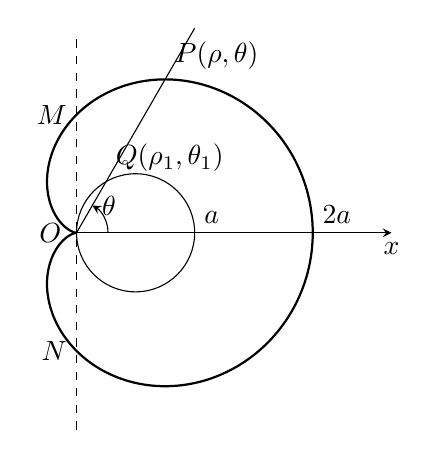
\begin{tikzpicture}[>=stealth]
\node[left=2pt]{$O$};
\draw[domain=0:180, smooth, thick, samples=100]plot({1.5*(cos(\x)+1)*cos(\x)}, {1.5*(cos(\x)+1)*sin(\x)});
\draw[domain=0:180, smooth, thick, samples=100]plot({1.5*(cos(\x)+1)*cos(\x)}, {-1.5*(cos(\x)+1)*sin(\x)});
\draw[fill=white](.75,0) circle(.75);
\draw[->](0,0)--(4,0)node[below]{$x$};
\draw[dashed](0,-2.5)--(0,2.5);
\node at (0,-1.5) [left]{$N$};
\node at (0,1.5)[left]{$M$};
\node at (1.5,0)[above right]{$a$};
\node at (3,0)[above right]{$2a$};
\draw(0,0)--(60:3);
\node at (60:.75)[above right]{$Q(\rho_1,\theta_1)$};
\node at (60:1.5+.75)[above right]{$P(\rho,\theta)$};
\draw[->](.4,0)arc (0:60:.4)node[right]{$\theta$};

\end{tikzpicture}
\captionof{figure}{}
\end{minipage}


这就是点$P$的轨迹的极坐标方程．它的曲线如图5.23所示，叫做\textbf{心脏线}.
\end{solution}



\begin{example}
    动点$M$在射线$\ell$上从$M_0$出发，以速度$v$远离点$O$作匀速运动，同时射线$\ell$又以角速度$\omega$逆时针绕射线的端点$O$作匀速转动（图5.24），求点$M$的轨迹．
\end{example}

\begin{solution}
    以点$O$为极点，射线$\vv{OM_0}$为极轴，建坐标系. 此时$M_0$的极坐标为$(\rho_0,0)$．设经过时刻$t$，动点在$\ell$上运动到$M$处，$\ell$转过了$\theta$角，则
\begin{equation}
\begin{cases}
    \theta=\omega t\\
    \rho=|OM_0|+vt=\rho_0+vt & (t\ge 0)
\end{cases} \tag{1}
\end{equation}

\noindent
\begin{minipage}{.6\textwidth}
    这就是动点$M$运动的参数方程（$t$为参数）. 消去$t$，得
    \begin{equation}
        \rho=\rho_0+\frac{v}{\omega}\theta \tag{2}
    \end{equation}
    若记$a=\frac{v}{\omega}$，它是一个常数，则(2)可写成
    \begin{equation}
        \rho=\rho_0+a\theta  \tag{3}
    \end{equation}
    它是点$M$轨迹的极坐标方程.
\end{minipage}
\hfill
\begin{minipage}{.35\textwidth}
\centering
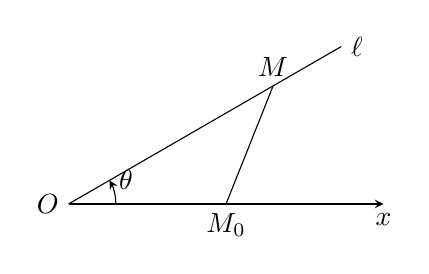
\begin{tikzpicture}[>=stealth]
\draw[->](0,0)node[left]{$O$}--(4,0)node[below]{$x$};
\draw(0,0)-- (30:4)node[right]{$\ell$};
\draw(30:3)node[above]{$M$}--(2,0)node[below]{$M_0$};
\draw[->](.6,0) arc (0:30:.6)node[right]{$\theta$};
\end{tikzpicture}
\captionof{figure}{}
\end{minipage}



应该注意：(3)中$\rho$是$\theta$的一次函数，在特殊情况下，当$\rho_0=0$，即动点初始位置$M_0$和定点$O$重合时，(3)变为
\begin{equation}
    \rho=a\theta  \tag{4}
\end{equation}
其中$\rho$变成$\theta$的正比例函数了.

现在，画出(4)的图形. 在极坐标系中画曲线的基本方法仍然是\textbf{描点法}. 先列表. 对于(4)，若$(\rho,\theta)$是其曲线上一点，则$(-\rho,-\theta)$也是曲线上的点，所以曲线对称于直线$\theta=\frac{\pi}{2}$. 从而，列表时只要列出$\theta\ge 0$的部分即可（$\theta\le 0$时，由对称性可简化作图）.

\begin{center}
\begin{tabular}{c|cccccccccc}
\hline
    $\theta$ & 0 &$\frac{\pi}{4}$& $\frac{\pi}{2}$& $\frac{3\pi}{4}$& $\pi$& $\frac{5\pi}{4}$& $\frac{3\pi}{2}$ & $\frac{7\pi}{4}$ & $2\pi$ & $\cdots$ \\
    \hline
$\rho$ & 0 &$\frac{\pi}{4}a$& $\frac{\pi}{2}a$& $\frac{3\pi}{4}a$& $\pi a$& $\frac{5\pi}{4}a$& $\frac{3\pi}{2}a$ & $\frac{7\pi}{4}a$ & $2\pi a$ & $\cdots$ \\
\hline
\end{tabular}
\end{center}

描出对应点（这里，我们画的是$a>0$的情形），依次用光滑曲线连接它们，便得到图5.25中的实线表示出的曲线．然后，再作出它关于直线$\theta=\frac{\pi}{2}$对称的曲线（虚线表示的部分）. 这样就得到了方程(4)的曲线.

方程(3)的曲线称为\textbf{等速螺线}（又称\textbf{阿基米德螺线}）．图5.25是它的特殊情况（$\rho_0=0$时）.

\noindent
\begin{minipage}{.4\textwidth}
\centering
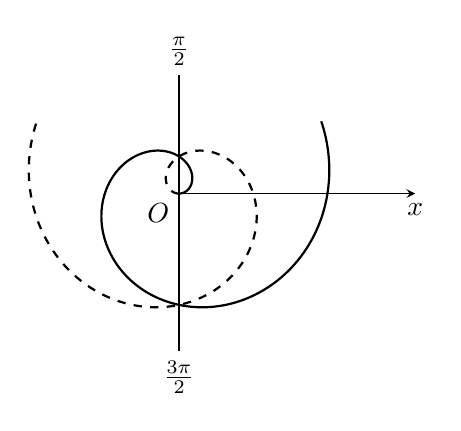
\begin{tikzpicture}[>=stealth]
\draw[->](0,0)--(3,0)node[below]{$x$};
\draw(0,-2)node[below]{$\frac{3\pi}{2}$}--(0,1.5)node[above]{$\frac{\pi}{2}$};
\node[below left]{$O$};
\draw[domain=0:2.15*pi, thick, smooth, samples=200]plot({.3*\x*cos(\x r)}, {.3*\x*sin(\x r)});
\draw[domain=0:2.15*pi, thick, smooth, samples=200, dashed]plot({-.3*\x*cos(\x r)}, {.3*\x*sin(\x r)});




\end{tikzpicture}
\captionof{figure}{}
\end{minipage}
\hfill
\begin{minipage}{.55\textwidth}
\centering
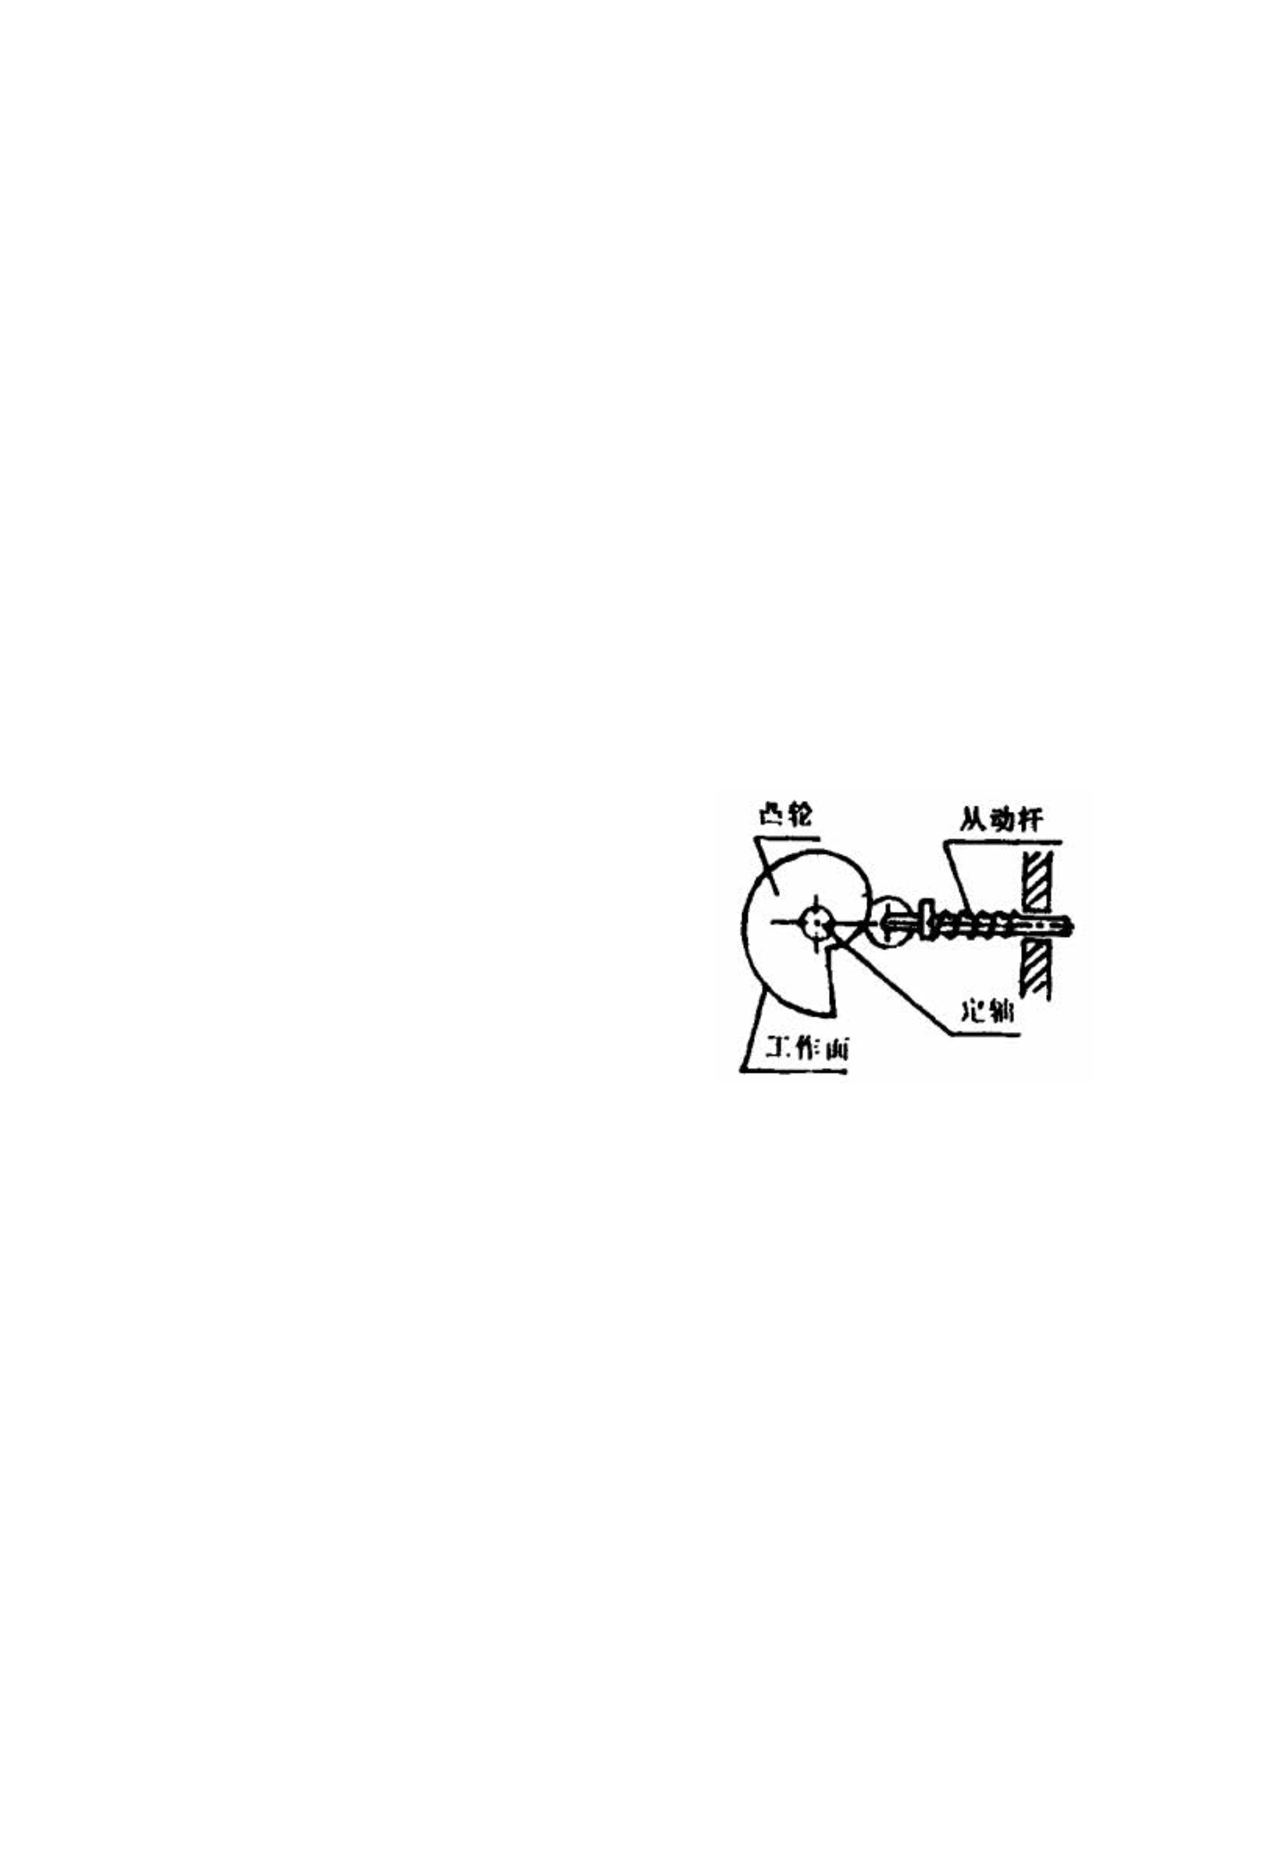
\includegraphics{fig/5-26.pdf}
\captionof{figure}{}
\end{minipage}

在机械传动时，常常利用凸轮把等速转动转化成等速直线运动．如图5.26，当凸轮绕定轴旋转时，它推动从动杆作左右往复直线运动.

在设计中，根据从动杆运动的不同要求，就要有不同的凸轮轮廓线. 因此，需求出轮廓线的方程. 有些凸轮轮廓线用等速螺线.
\end{solution}


\begin{example}
由于某种需要，设计一个凸轮，轮廓线如图5.27所示，要求如下：

凸轮依顺时针方向绕点O转动，开始时从动杆接触点为$A$，$|OA|=4$cm.
\begin{enumerate}
\item 当从动杆接触轮廓线$ABC$时，它被推向右方作等速直线运动. 凸轮旋转角度$\frac{11}{8}\pi$时，有最大推程18cm，即$|OC|=18$cm;
\item 当从动杆接触轮廓线$CDA$时，它向左等速退回原位.
\end{enumerate}

求曲线$ABC$和曲线$CDA$的方程.
\end{example}

\begin{solution}
取极坐标系，如图5.27．

由已知可知，所求两段曲线都是等速螺线. 设曲线$ABC$的方程为
\begin{equation}
    \rho=\rho_0+a\theta \tag{1}
\end{equation}

\noindent
\begin{minipage}{.6\textwidth}
$\because\quad A(4,0)$和$C\left(18,\frac{11}{8}\pi\right)$都在曲线(1)上

$\therefore\quad \begin{cases}
    4=\rho_0 \\ 18=\rho_0+a\cdot \frac{11}{8}\pi
\end{cases}$解之，得
\[\rho_0=4,\qquad a=\frac{112}{11\pi}\]
代入(1)，得到曲线$ABC$的极坐标方程为
\[\rho=4+\frac{112}{11\pi}\theta\quad \left(0\le \theta\le \frac{11}{8}\pi\right)\]
\end{minipage}
\hfill
\begin{minipage}{.37\textwidth}
\centering
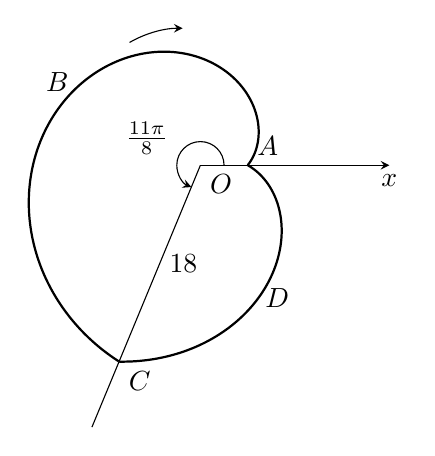
\begin{tikzpicture}[>=stealth, scale=.3]
\draw[->](0,0)--(8,0)node[below]{$x$};
\node[below right]{$O$};
\draw[domain=0:11*pi/8, thick, smooth, samples=200]plot({(2+1.62*\x)*cos(\x r)}, {(2+1.62*\x)*sin(\x r)});
\draw[domain=11*pi/8:2*pi, thick, smooth, samples=200]plot({(24.4-3.565*\x)*cos(\x r)}, {(24.4-3.565*\x)*sin(\x r)});
\node at (2,0)[above right]{$A$};
\draw(0,0)--node[right]{18}(247.5:9)node[below right]{$C$}--(247.5:12);
\draw[->](1,0) arc (0:247.5:1);
\node at (130:1.5)[left]{$\frac{11\pi}{8}$};
\node at (150:7){$B$};
\node at (-60:6.5){$D$};
\draw[->](120:6)arc (120:90:4.5);

\end{tikzpicture}
\captionof{figure}{}
\end{minipage}

再设曲线$CDA$的方程为
\begin{equation}
    \rho=\rho_1+a_1\theta \tag{2}
\end{equation}

$\because\quad $点$C\left(18,\frac{11}{8}\pi\right)$和$A(\pi,2\pi)$都在曲线(2)上

$\therefore\quad \begin{cases}
    18=\rho_1+a_1\cdot \frac{11\pi}{8}\\
    4=\rho_1+a_1\cdot 2\pi
\end{cases}$解之，得
\[\rho_1=48.8,\qquad a_1=-\frac{22.4}{\pi}\]
代入(2)，得到曲线$CDA$的极坐标方程为
\[\rho=48.8-\frac{22.4}{\pi}\theta\quad \left(\frac{11}{8}\pi\le \theta\le 2\pi\right)\]
\end{solution}





\subsection*{5.4 练习}
\begin{enumerate}
    \item 由定点$O$向定直线$\ell$引射线$OM$交$\ell$于$M$，延长$OM$至$P$，使$|MP|=a\; (a>0)$，若直线$\ell$的方程为$\rho\cos\theta=5$，则$M$在$\ell$上移动时，求点$P$的轨迹方程.
    \item 设$O$为坐标原点，$P$是圆$x^2+y^2+2ax=0\; (a<0)$上的一点，$Q$是射线$OP$上的一点，且满足$|OP|\cdot |OQ|=a^2$，当$P$在圆上移动时，求点$Q$的轨迹.
    \item 对于曲线$\rho=\frac{2}{1+\cos\theta}$，过其极点$O$作弦$AB$，试求$|AB|$的最小值.
    \item 求证：如果$M_1(\rho_1,\theta_1)$、$M_2(\rho_2,\theta_2)$是等速螺线上的两个点，则$\rho_2-\rho_1$与$\theta_2-\theta_1$成正比例.
    \item 某自动机床上有一个凸轮. 它的轮廓线中有一段$ACB$是等速螺线（如图）. 点$O$是旋转中心，$|OA|=\rho_0=60$毫米，轴心角$\angle AOB=30^{\circ}$. 工作时，曲线$ACB$能把从动杆推出5毫米. 求曲线$ACB$的方程.

    \begin{center}
\begin{tikzpicture}[>=stealth]
\begin{scope}[scale=1.2]
    \draw[domain=0:pi/6, thick, smooth, samples=100]plot({(1.25+1.0/pi*\x)*cos(\x r)}, {(1.25+1.0/pi*\x)*sin(\x r)});
    \draw[domain=pi/6:2*pi, thick, smooth, samples=100]plot({(1.25+1/6-0.028937*\x)*cos(\x r)}, {(1.25+1/6-0.028937*\x)*sin(\x r)});
\draw(1.25,0)node[right]{$A$}--(0,0)node[below]{$O$}--(30:1.25+1/6)node[right]{$B$};
\draw(.4,0) arc (0:30:.4)node[right]{$30^{\circ}$};
\draw[->](80:1.6) arc (80:40:1.6);
\node at (15:1.6){$C$};
\node at (0,-2){第5题};
\end{scope}    
\begin{scope}[xshift=6cm, scale=.4]

\draw[domain=0:pi/2, thick, smooth, samples=100]plot({(2.5+2.0/pi*\x)*cos(\x r)}, {(2.5+2.0/pi*\x)*sin(\x r)});
\draw[domain=90:240, thick, smooth, samples=100]plot({(3.5)*cos(\x)}, {(3.5)*sin(\x)}); 
\draw[domain=4*pi/3:2*pi, thick, smooth, samples=100]plot({(3.5-1.5/pi*(\x-4*pi/3))*cos(\x r)}, {(3.5-1.5/pi*(\x-4*pi/3))*sin(\x r)});
\draw(0,3.5)node[above]{$B$}--(0,0)node[below]{$O$}--(2.5,0)node[below left=3pt]{$A$};
\draw(0,0)--(-120:3.5)node[below]{$C$};
\draw[->](1,0) arc (0:240:1)node[above left]{$\frac{4\pi}{3}$};
\draw(0,0) rectangle(.4,.4);
\draw[pattern=north east lines](2.5+.3,-.3) rectangle (6,.3);
\draw[fill=white](2.5+.3,0)circle (.3);
\draw[fill=white](2.5+.3,0)circle (.1);
\node at (0,-6){第6题};

\end{scope}  
\end{tikzpicture}    
\end{center}

\item 如图为一个凸轮，由三段不同的曲线组成：当$\theta\in\left[0,\frac{\pi}{2}\right]$时，曲线$AB$是等速
    螺线；当$\theta\in\left[\frac{\pi}{2},\frac{4\pi}{3}\right]$时，曲线$BC$是$\theta\in\left[\frac{\pi}{2},2\pi\right]$时，曲线$BC$是
    一段圆弧；当$\theta\in\left[\frac{4\pi}{3},2\pi\right]$时，曲线$CA$
    也是一段等速螺线. 已知$|OA|=25$, $|OB|=35$，试求出曲线$AB$、$BC$、$CA$的极坐标方程.
    \item 已知等速螺线经过两个点$A\left(22,\frac{\pi}{6}\right)$，$B(44,2\pi)$. 求出这个螺线的方程，并画出$\theta\in [0,2\pi]$时的图形.
    \item 证明方程$\rho=\frac{C}{1+a\cos\theta+b\sin\theta}$
    的曲线是圆锥曲线. 在什么条件下是椭圆？双曲线？抛物线？
    \item 已知抛物线的焦点在极坐标系的极点，抛物线的主轴垂直极轴，且抛物线过$\left(1,-\frac{\pi}{2}\right)$点，写出抛物线的方程.
    \item $\triangle ABC$三个顶点的极坐标分别为$A\left(9,\frac{\pi}{10}\right)$、$B\left(12,\frac{4\pi}{15}\right)$、$C\left(10,\frac{3\pi}{5}\right)$，求这个三角形的面积.
    \item 在极坐标系中，求
\begin{enumerate}[(1)]
    \item $A\left(8,-\frac{2\pi}{3}\right)$、$B\left(6,\frac{\pi}{3}\right)$的中点$M$的极坐标； 
    \item $C\left(4,\frac{\pi}{6}\right)$、$D\left(6,\frac{\pi}{2}\right)$之间的距离$|CD|$.
\end{enumerate}

\item 求曲线$\rho=\frac{3}{2-2\cos\theta}$与$\rho=6\cos\theta$的交点.
\item $F$为椭圆$\frac{x^2}{8}+\frac{y^2}{4}=1$的一焦点，它的坐标是非负数，$P$为椭圆上的动点，连$FP$，延长至$M$，使$FM:FP=3:2$，求点$M$的轨迹方程.
\end{enumerate}

\section{本章小结}
\subsection{知识结构与常用解题方法}
\begin{center}
    \begin{tikzpicture}[>=stealth]
\node[draw] (A) at (0,0)[text width=1.7cm, align=center]{极坐标的\\基本思想};
\node[draw] (A1) at (3,0)[text width=1.7cm, align=center]{极坐标系\\（多值性）};
\node[draw] (A2) at (6.5,0)[text width=3cm, align=center]{极坐标系中\\曲线与方程的定义};
\node[draw] (A3) at (10,0)[text width=2cm, align=center]{曲线极坐标\\方程的求法};
\draw[->, thick](A)--(A1);
\draw[->, thick](A1)--(A2);
\draw[->, thick](A2)--(A3);
    \end{tikzpicture}
\end{center}

\begin{enumerate}[(1)]
\item 直接法：把极径、极角与已知条件集中在一个三角形中解之.
\item 定义法：对于熟知的曲线，只要求出方程中的未定系数即可.
\item 参数法：相关点轨迹问题的一般解法（选参、用参、消参）.
\end{enumerate}

\subsection{常见曲线的极坐标方程}
\begin{center}
\begin{tabular}{c|cc}
\hline
& 一般方程 & 特殊情况\\
\hline
&& $\theta=\theta_0\; (\rho\in\R)$  \\
直线& $\rho\cos(\theta-\omega)=p\quad (p>0)$  & $\rho\cos\theta=\pm p$\\
&&$\rho\sin\theta=\pm p\quad (p>0)$\\
\hline
圆& $r^2=\rho^2+\rho^2_0-2\rho\rho_0\cos(\theta-\theta_0)$  &  $\rho=r$ （圆心在极点） \\
&& $\rho=2r\cos(\theta-\theta_0)$（圆过极点时）\\\hline
抛物线\\
椭圆& $\rho=\frac{ep}{1-e\cos\theta}$  &   \\
双曲线\\\hline
等速螺线& $\rho=\rho_0+a\theta$  &  $\rho=a\theta$ \\
\hline

\end{tabular}
\end{center}

\subsection{极坐标方程与普通方程的互化}
\[P(\rho,\theta)\xrightleftharpoons[\text{用图示法}]{\text{用公式(1)}} P(x,y)\]
\[\varphi(\rho,\theta)=0\xrightleftharpoons[\text{用公式(1)}]{\text{凑出}\rho\cos\theta, \; \rho\sin\theta} f(x,y)=0\]

\subsection{几点说明}
\begin{enumerate}
  \item 对极坐标系，它与直角坐标系的根本区别在于点的极坐标的多值性.
\item 对曲线的极坐标方程的定义，要弄清与直角坐标方程的区别和原因.
\item 对熟知曲线的方程，要理解其中每个字母的几何意义是什么？公式是如何导出的？
\item 对于极坐标方程与普通方程的互化，要明确互化的三条前提、互化的方法和互化的功能.
\end{enumerate}

\section*{复习题三}
\begin{center}
    \bfseries A
\end{center}

\begin{enumerate}
    \item 极坐标方程$\rho\cos\left(\theta-\frac{\pi}{3}\right)=2$表示什么曲线？
    \item 求两圆$\rho=\cos\theta$与$\rho=\sin\theta$的圆心距.
    \item 正方形两个相对顶点的极坐标分别为$\left(6,-\frac{7\pi}{12}\right)$和$\left(4,\frac{\pi}{6}\right)$，求正方形的面积.
    \item 在极坐标系中，求点$\left(2,-\frac{\pi}{6}\right)$到直线$\rho\sin(\theta-30^{\circ})=1$的距离.
    \item 判断下面两直线的位置关系：
\begin{enumerate}[(1)]
    \item $\rho\sin \left(\theta-\frac{\pi}{3}\right)=2$和$\tan\theta=-\frac{\sqrt{3}}{3}$
    \item $\rho\sin \left(\theta+\frac{2\pi}{9}\right)=5$和$\rho\cos\left(\theta-\frac{5\pi}{18}\right)=3$
\end{enumerate}
\item 化下列极坐标方程为直角坐标方程：
\begin{multicols}{2}
 \begin{enumerate}[(1)]
    \item $\rho^2\cos 2\theta=4$
    \item $3\rho\cos\theta-5\rho+16=0$
    \item $\rho=4\cot\theta \csc\theta$
\end{enumerate}   
\end{multicols}

\item 若极坐标方程$\rho=\frac{4}{2-\kappa\cos\theta}$表示椭圆，求$\kappa$的取值范围.
\item 曲线的极坐标方程为$\rho=\frac{5}{3-2\cos\theta}$，求它的焦点坐标。
\item 求椭圆$\rho=\frac{1}{3-2\sqrt{2}\cos\theta}$的长轴长和两条准线的极坐标
方程.
\item 求以$\rho=\frac{\sqrt{3}}{\sqrt{3}-2\cos\theta}$为方程的双曲线的两条渐近线的夹角.
\item 画出极坐标方程$(1-2\cos\theta)\rho^2-(\cos\theta-\cos2\theta)\rho+\cos\theta=0$所表示的曲线．
\item 等速螺线共有三圈，螺线上距旋转中心的最近距离是
20cm，最远距离是35cm，求其极坐标方程。
\end{enumerate}


\begin{center}
    \bfseries B
\end{center}

\begin{enumerate}\setcounter{enumi}{12}
    \item $F$是定点，$\ell$是定直线. 点$F$到直线$\ell$的距离为$p\; (p>0)$，点$M$在直线$\ell$上滑动，动点$N$在$MF$的延长线上，且满足条件$\frac{|FN|}{|MN|}=\frac{1}{|MF|}$
\begin{multicols}{2}
\begin{enumerate}[(1)]
    \item 求动点$N$的轨迹；
    \item 求$|MN|$的最小值．
\end{enumerate}
\end{multicols}
\end{enumerate}
